\documentclass[abstracton,12pt,oneside]{scrreprt}

\usepackage[utf8]{inputenc}
\usepackage[T1]{fontenc}
\usepackage{fancyhdr}
\usepackage{graphicx}
\usepackage{tikz}
\usetikzlibrary{matrix}
\usepackage{times}
\usepackage{listings}
\usepackage{amssymb}
\usepackage{amsfonts}
%\usepackage{algorithm}
\usepackage{algpseudocode}
\usepackage{mathtools}
\usepackage{amsmath}
\usepackage{url}
\usepackage{chapterbib}
\usepackage{gensymb}
\usepackage{BTree}
\usepackage{weiwBTree}
\usepackage{float}
\usepackage{array}
\usetikzlibrary{shapes, calc}
\usepackage[ruled,linesnumbered,lined,commentsnumbered]{algorithm2e}
\usepackage{pgfplots}
\usepackage[titletoc]{appendix}

\DeclarePairedDelimiter\ceil{\lceil}{\rceil}
\DeclarePairedDelimiter\floor{\lfloor}{\rfloor}

\setlength{\parindent}{0pt} 


\titlehead{Department of Informatics, University of Zurich}
\subject{\vspace*{2cm}BSc Thesis}
\title{Implementing an Index Structure for Streaming Time Series Data}
\author{
  Melina Mast\\[-5pt]
  \scriptsize Matrikelnummer: 13-762-588\\[-5pt]
  \scriptsize Email: \texttt{melina.mast@uzh.ch}
}
\date{\vspace*{2cm}August, 2016}
\publishers{
  \small supervised by Prof.\ Dr.\ Michael Böhlen and Kevin Wellenzohn \\[5cm]
  \begin{tikzpicture}[overlay]
    \node at (-3,-3) {
\includegraphics[height=5.5cm]{IFIlogo}};
    \node at (7,-3) {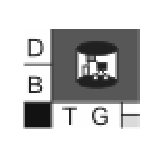
\includegraphics[height=2cm]{dbtgBW}};
  \end{tikzpicture}
}

%\dedication{dedicated to my family}

% --------- 

\newtheorem{definition}{Definition}
\newtheorem{example}{Example}
\newtheorem{theorem}{Theorem}
\newtheorem{lemma}{Lemma}

\newenvironment{proof}
  {\noindent{\bf Proof:\rm}}{\hfill$\Box$\vspace{\medskipamount}}

\def\bbbr{{\rm I\!R}}
\def\bbbm{{\rm I\!M}}
\def\bbbn{{\rm I\!N}}
\def\bbbz{{\rm I\!Z}}

% --------- 

\begin{document}


\maketitle

\chapter*{Acknowledgements}



\begin{abstract}
A streaming time series is an unbounded sequence of data points that is continuously extended. The data points arrive in a predefined interval (e.g. every 5 minutes). \\Such time series are relevant to applications in diverse domains. Imagine a meteorology station that sends a temperature measurement every 3 minutes or imagine a trader in the financial stock market who receives updated pricing information every 5 minutes.\\
We present an implementation of an index structure for streaming time series data. The system keeps a limited amount of time series data in main memory. As a result, it is able to access the information of past measurements in time window $W$. We introduce an implementation using two data structures, a circular array and a $B^+$tree, to efficiently access the data of past measurements. 

\end{abstract}

\chapter*{Zusammenfassung}
Kontinuierliche Zeitreihen werden durch neu ankommende Daten unbegrenzt erweitert. Die Daten werden in einem vordefinierten Intervall aktualisiert.\\
Derartige Zeitreihen sind relevant für diverse Bereiche. Beispielsweise in der Meteorologie, in welcher die Wetterinformationen kontinuierlich aktualisiert werden oder, um einen weiteren Bereich zu nennen, in Finanzmärkten, wo die Händler auf die neusten Preisinformationen angewiesen sind.\\
Wir präsentieren die Implementation einer Indexstruktur für kontinuierlich erweiterte Zeitreihen. Unser System behält eine limitierte Anzahl an vergangenen Daten im Arbeitsspeicher. Daraus resultiert, dass das System auf vergangenen Daten zugreifen kann. Dazu stellen wir unsere Implementation vor, welche von zwei Datenstrukturen Gebrauch macht: einem zirkulären Array und einem $B^+$baum. Die beiden Datenstrukturen erlauben den effizienten Zugriff auf alle Werte der vergangenen Daten, welche sich noch im Zeitfenster befinden.

\tableofcontents
\listoffigures
\listoftables
\listofalgorithms
\renewcommand{\lstlistingname}{Algorithm}% Listing . Algorithm
\renewcommand{\listtablename}{Tables}

\addtocontents{loa}{\def\string\figurename{Algorithm}}

%todo check macht es silbentrennung automatisch korrekt?
\chapter{Introduction}
A streaming time series is an unbounded sequence of data points that is continuously extended, potentially forever. The data points arrive in a predefined interval (e.g. every 5 minutes). Such time series are relevant to applications in diverse domains. Imagine a meteorology station that sends a temperature measurement every 3 minutes or imagine a trader in the financial stock market who depends on updated pricing information. Thus, various applications need to be fed continuously with the latest data. \\
Our system neither forgets about and deletes all past measurements nor keeps all of them, since a system can only keep a limited size of data in main memory. But because a portion of the data is kept, it is still possible to access past data. The system provides data structures and operations to efficiently access the time point and the value of a measurement.\\
The thesis proposes an implementation for an index structure for streaming time series data. In order to achieve efficient access to the time points and values of  measurements, the system uses two data structures: A circular array in combination with a $B^+$tree. The circular array has a limited size. The measurements are stored in the array, sorted by time. The $B^+$tree as well contains the same measurements with time points in a predefined sliding time window. The leaves of the tree are sorted from left to right by the measurement value. Thus, range queries can be efficiently performed. For every new measurement the time window slides forward. A value drops out of the window and a new value is inserted to the circular array and the $B^+$tree. If a measurements time point is not in the sliding window any more, it is deleted from both data structures. 
\\The introduced system is not only implemented but also analysed in terms of space and runtime complexity. Further, an experimental evaluation tries to underpin the theoretical results.
\\ \\
At the beginning of this thesis, in chapter \ref{background}, the TKCM algorithm designed by Wellenzohn et al.\cite{BScT} is introduced. To achieve a better understanding for the system context and for the requirements our system must satisfy. Chapter \ref{ProblemDefinition} describes the context and introduces the operations that our system must be able to perform. In chapter \ref{sec:Approach}, our approach is represented and its advantages are discussed. Further, the pseudo-code for implementing the system is outlined. After that, the runtime and space complexity of the implementation is described in chapter \ref{Complexity}. Followed by an experimental evaluation of the implemented system in chapter \ref{sec:Experimental}. Finally, the thesis is summed up in chapter \ref{sec:Summary}.


\newtheorem{defn}{Definition}[section]
\newtheorem{exmp}{Example}[section]
\newcommand*{\argmin}{\operatornamewithlimits{argmin}\limits}

\chapter{Background}
\label{background}
A streaming time series is not always gapless. Due to sensor failures or transmission errors, values can get missing. To efficiently recover missing values, Wellenzohn et al.\cite{BScT} present the Top-$k$ Case Matching algorithm (TKCM). The algorithm and its connection to this thesis is introduced in Section \ref{TKCM}.

\section{TKCM}
\label{TKCM}
TKCM monitors a set of streaming time series and imputes missing measurement values if it detects any. It defines a two-dimensional query pattern over the most recent values of a set of time series. The idea is to derive a missing value in time series $s$ from the \emph{k} most similar past pattern. For each \emph{time series} $s$ a set of highly correlated \emph{reference time series} are determined. Such that TKCM is able to recover a missing value in streaming time series data.

\begin{defn}
	(Time Series) Let $S$ be a set $S = \{s_1,s_2,...\}$ of streaming time series. The measurement value of time series $s \in S$ at time \emph{t} is denoted as $s(t)$. For base time series $s$, let $R_s = \langle r_1, r_2,...\rangle$ be an ordered sequence of the time series $r_i \in S \setminus \{s\}$. The set of $\text{reference time series}$ for $s$, $R_s^d$, at the current time $\bar{t}$ are the first $d$ time series in $R_s$ for which $r(\bar{t}) \neq \text{NIL}$.
	The time points in a streaming time series $s$ are in time window $W$. 
	The measurement value of a time series $s \in S$ at time point $t_i$ is denoted as $s_i(t)$. Hence, a measurement is represented by the tupel $(t, s_i(t))$.
\end{defn}

To be able to recover a missing measurement value, TKCM retains a sliding window of the streaming time series in main memory. 

\begin{defn}
	(Sliding Window) Let $W=[ \underline{t}, \bar{t} ]$ be a sliding window of length $|W|$. Time $\underline{t}$ represents the oldest time point that fits into the time window and time $\bar{t}$ represents the most recent time point for which the stream produced a new value. 
\end{defn}
To impute a missing value, TKCM defines a query pattern $Q(\bar{t})$ over the most recent values of the reference time series. Afterwards, TKCM looks for the \emph{k} most similar patterns in the sliding window.  
\begin{figure}[H]
	\centering
	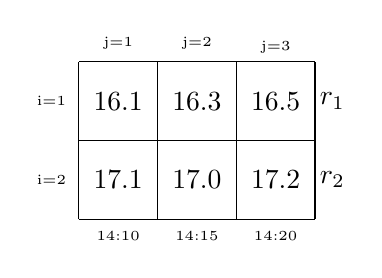
\begin{tikzpicture}
	\definecolor{mycolor}{RGB}{224,224,224}
	\definecolor{mycolor2}{RGB}{192,192,192}
	\draw[step=1cm,color=black] (0,0) grid (3,2);
	\node at (0.5,+0.5) [label={[font=\tiny,label distance=0.3cm]below:$\text{14:10}$}, label={[font=\tiny,label distance=0.1cm]left:$\text{i=2}$}]{17.1};
	\node at (1.5,+0.5) [label={[font=\tiny,label distance=0.3cm]below:$\text{14:15}$}]{17.0};
	\node at (2.5,+0.5) [label=right:$r_2$,label={[font=\tiny,label distance=0.3cm]below:$\text{14:20}$}]{17.2};
	\node at (0.5,+1.5) [label={[font=\tiny,label distance=0.3cm]above:$\text{j=1}$}, label={[font=\tiny,label distance=0.1cm]left:$\text{i=1}$}]{16.1};
	\node at (1.5,+1.5) [label={[font=\tiny,label distance=0.3cm]above:$\text{j=2}$}]{16.3};
	\node at (2.5,+1.5) [label=right:$r_1$,label={[font=\tiny,label distance=0.25cm]above:$\text{j=3}$}]{16.5};	
	\end{tikzpicture}
	\caption{Example of a query pattern Q(t) of length $l=3$ and $d=2$ reference time series.}
\end{figure}
\begin{defn}
	(Pattern) Let $R_s^d=\{r_1,...,r_d\}$ be the ordered set of reference time series for a time series $s$. A $pattern$ $P(t)$ of length $l > 0$ over $R_s^d$ that is embedded at time $t$ is defined as a $d\times l$ matrix $P(t) = [p_{i,j}]_{d\times l}$ where $p_{i,j}=S_i(t-j+l)$. $P(t)$ is a set of pattern cells $p_{i,j}$, such that $p_{i,j}$ $\in P(t)$. 
\end{defn}
The two-dimensional query pattern $Q(\bar{t})$ is anchored at a time point $\bar{t}$ and consists of the subsequence of length $l$ spanning from $(\bar{t}-l+1$ to $\bar{t})$ of each reference time series. Each row represents a subsequence of a reference time series and each column represents the values of the reference time series at a time point.\\ 
Only the values in the streaming time series with time points in time window $W$ are kept in main memory. $\forall t: \underline{t} \leq t < \bar{t} \rightarrow s(t) \ne \text{NIL}$ since \emph{s} contains imputed values if the real ones are missing. \\
TKCM  initializes one neighborhood $N(q_{i,j})$ around each $q_{i,j} \in Q(\bar{t})$. The algorithm continuously looks up new candidate pattern $P(t)$ in the time window $t \in W$ by \emph{growing} the neighborhoods $N(q_{i,j})$ until it found the $k$ most similar patterns to $Q(\bar{t})$. It remembers the time points $t$ in a set $T$ to avoid considering these patterns again. 
\begin{defn}
		\label{def3}
	(Next Pattern) The next pattern for neighborhood $N(q_{i,j})$ is pattern $P(t) = [p_{i,j}]_{d\times l}$ anchored at time point $t = \argmin_{t \in W \setminus T} |p_{i,j}-q_{i,j}|$
\end{defn}
TKCM must not only impute missing values, but also process the new measurements efficiently. Therefore, TKCM must provide an insertion method for new arriving values to insert them into a streaming time series $s$. Since the time window has a limited, given size $|W|$, one value has to be deleted from the time series data for each new arriving value. Provided that, the time series data in window $W$ is already completely filled. 


\section{Access Methods}
\label{AccessMethods}
The Next Pattern (Def. \ref{def3})  is built on top of two access methods.\emph{Sorted} access is used to find the most similar value to a given query pattern cell $q_{i,j}$ and \emph{random} access retrieves the values to fill the remaining pattern cells. The two methods are defined as follows: 
%check if follows or followed
\begin{defn}
	\label{sorted}
	(Sorted Access) Sorted access for a neighborhood $N(q_{i,j})$ returns the next yet unseen measurement $(t, s_i(t))$ where $t = \argmin_{t \in W \setminus T} |s_i(t) - q_{i,j}|$.
\end{defn}
\begin{defn}
	\label{random}
	(Random Access) Random access returns value r(t), given time series r and time point t.	
\end{defn}
\begin{figure}[H]
	\centering
	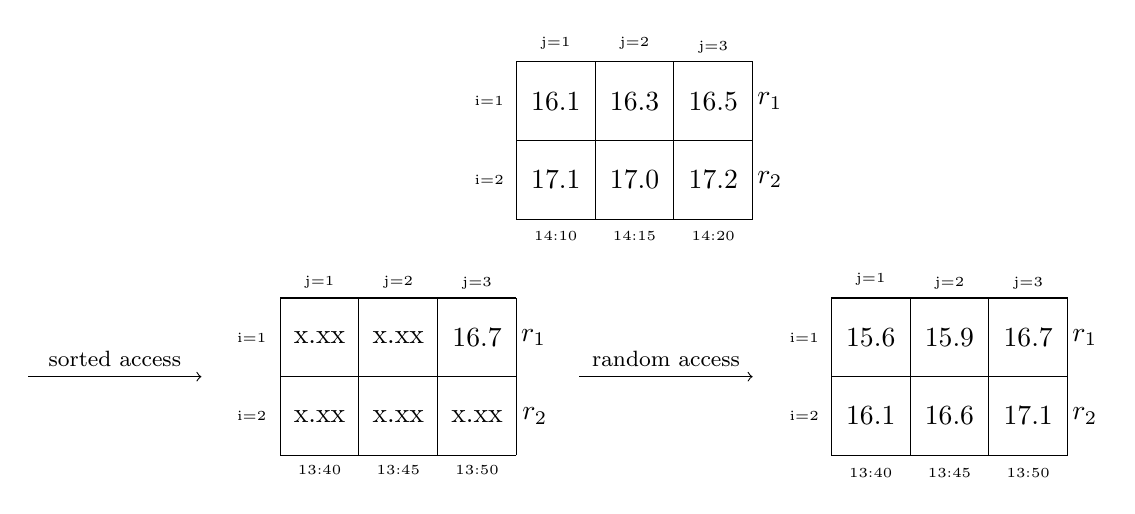
\begin{tikzpicture}
	\definecolor{mycolor}{RGB}{224,224,224}
	\definecolor{mycolor2}{RGB}{192,192,192}
	\draw[step=1cm,color=black] (3,3) grid (6,5);
	\node at (3.5,+3.5) [label={[font=\tiny,label distance=0.3cm]below:$\text{14:10}$}, label={[font=\tiny,label distance=0.1cm]left:$\text{i=2}$}]{17.1};
	\node at (4.5,+3.5) [label={[font=\tiny,label distance=0.3cm]below:$\text{14:15}$}]{17.0};
	\node at (5.5,+3.5) [label=right:$r_2$,label={[font=\tiny,label distance=0.3cm]below:$\text{14:20}$}]{17.2};
	\node at (3.5,+4.5) [label={[font=\tiny,label distance=0.3cm]above:$\text{j=1}$}, label={[font=\tiny,label distance=0.1cm]left:$\text{i=1}$}]{16.1};
	\node at (4.5,+4.5) [label={[font=\tiny,label distance=0.3cm]above:$\text{j=2}$}]{16.3};
	\node at (5.5,+4.5) [label=right:$r_1$,label={[font=\tiny,label distance=0.25cm]above:$\text{j=3}$}]{16.5};	

\definecolor{mycolor}{RGB}{224,224,224}
\definecolor{mycolor2}{RGB}{192,192,192}

\draw[->]  (-3.2,1) -- (-1,1) node [pos=0.5,above,font=\footnotesize] {sorted access};

\draw[step=1cm,color=black] (0,0) grid (3,2);
\node at (0.5,+0.5) [label={[font=\tiny,label distance=0.3cm]below:$\text{13:40}$}, label={[font=\tiny,label distance=0.1cm]left:$\text{i=2}$}]{x.xx};
\node at (1.5,+0.5) [label={[font=\tiny,label distance=0.3cm]below:$\text{13:45}$}]{x.xx};
\node at (2.5,+0.5) [label=right:$r_2$,label={[font=\tiny,label distance=0.3cm]below:$\text{13:50}$}]{x.xx};
\node at (0.5,+1.5) [label={[font=\tiny,label distance=0.3cm]above:$\text{j=1}$}, label={[font=\tiny,label distance=0.1cm]left:$\text{i=1}$}]{x.xx};
\node at (1.5,+1.5) [label={[font=\tiny,label distance=0.3cm]above:$\text{j=2}$}]{x.xx};
\node at (2.5,+1.5) [label=right:$r_1$,label={[font=\tiny,label distance=0.25cm]above:$\text{j=3}$}]{16.7};

\draw[->]  (3.8,1) -- (6.0,1) node [pos=0.5,above,font=\footnotesize] {random access};

\draw[step=1cm,color=black] (7,0) grid (10,2);
\node at (7.5,+0.5) [label={[font=\tiny,label distance=0.3cm]below:$\text{13:40}$}, label={[font=\tiny,label distance=0.1cm]left:$\text{i=2}$}]{16.1};
\node at (8.5,+0.5) [label={[font=\tiny,label distance=0.3cm]below:$\text{13:45}$}]{16.6};
\node at (9.5,+0.5) [label=right:$r_2$,label={[font=\tiny,label distance=0.3cm]below:$\text{13:50}$}]{17.1};
\node at (7.5,+1.5)[label={[font=\tiny,label distance=0.3cm]above:$\text{j=1}$}, label={[font=\tiny,label distance=0.1cm]left:$\text{i=1}$}]{15.6};
\node at (8.5,+1.5) [label={[font=\tiny,label distance=0.25cm]above:$\text{j=2}$}]{15.9};
\node at (9.5,+1.5) [label=right:$r_1$,label={[font=\tiny,label distance=0.25cm]above:$\text{j=3}$}] {16.7} ;


\end{tikzpicture}

\caption{Pattern for query pattern cell $q_{1,3}$.}
\end{figure}
The next pattern search is presented in algorithm \ref{NextPattern}. TKCM initializes a set $T =\{\}$. The set is filled during execution with all time points \emph{t} for which a pattern P(t) has been processed. 
Using the sorted access mode, the algorithm finds the next yet unseen time point $t \notin T$ for which the value is most similar to a given value in a query pattern cell $q_{i,j}$. The random access mode is used to look up the values that pattern $P(t)$ is composed of. 

\BlankLine
\begin{algorithm}[H]
	\IncMargin{1em}
	\SetAlgoLined
	\DontPrintSemicolon
	\KwIn{Neighborhood $N(q_{i,j})$ and seen time points $T$}
	\KwOut{Next pattern $P(t{'})$}

		P $\leftarrow$ matrix of size $d\times l$\;
		$(t, s_i(t))$ $\leftarrow$ sortedAccess(N($q_{i,j}$),$T$)\; 
		P[i,j] $\leftarrow$ $s_i(t)$\;	
		\ForEach{$q_{x,y}$ $ \in Q(\bar{t}) \setminus{q_{i,j}}$}
		{
		P[x,y] $\leftarrow$ randomAccess($s_x$, $t-y+j$)\;
		}
		\Return P anchored at time $t-j+l$\;
	
	
	\caption{NextPattern}
	\label{NextPattern}
\end{algorithm}


\chapter{Problem Definition}
\label{ProblemDefinition}
The present thesis introduces an implementation of the $random$ and $sorted$ access method for a streaming time series $s$. The access modes are described in the previous Section \ref{AccessMethods}. The required operations and the context for our system are presented in the following.

\section{Context}
%TODO check if for or to our system
We make the following assumptions for our system: 
\begin{itemize}  
	\item The measurements arrive in a fixed interval (E.g. every five minutes). 
	\item There are no gaps between the measurements since the gaps are filled before values are inserted in the data structure.
	\item There are no measurements that arrive out-of-order.
\end{itemize}


\section{Operations}
\label{sec:Op}
The system needs to efficiently perform on the streaming time series $s$ in a sliding window $W$: 
\begin{itemize}  
	\item shift$(\bar{t}, v)$: add value \emph{v} for the new current time point $\bar{t}$ and remove value \emph{v'} for the time point $\underline{t} - 1$ that just dropped out of time window $W$.
	\item sortedAccess$(v, T)$: given a value \emph{v} and a set of time points $T$, return the time point $t \not\in T$ such that $|v-s(t)|$ is minimal (Def. \ref{sorted}).
	\item randomAccess$(t)$: return the value of time series \emph{s} at time \emph{t}, denoted by $s(t)$ (Def. \ref{random}).
	\item newNeighborhood$(t,v,j,l)$: given a value \emph{v} for the time point $t$, the pattern length $l$ and the index $j$, return the new neighborhood $N$ at $t$.
\end{itemize}
Wellenzohn et al.\cite{BScT} suggest a combination of two data structures: a $B^+$tree and a circular array. The random access operation can be performed by the circular array, while the sorted access operation is executed on the leaves of a $B^+$tree. \\Additional reasons for the data structures are described in Chapter \ref{sec:Approach}. Further, the implementation of the random and sorted access modes using the suggested data structures is presented and a solution for  handling duplicate values is proposed. 



\chapter{Approach}
\label{sec:Approach}
Each time series $s \in S$ is represented by a circular array. The circular array is kept in main memory. It uses random access to look up value $s(t)$ for a given time $t$. Further, for each time series $s$ a $B^+$tree is maintained that is also kept in main memory. The $B^+$tree is ideal for sorted access by value and therefore for range queries. Both data structures are described in detail in Section \ref{sec:circularArray} and Section \ref{sec:BplusTree}, respectively. Figure \ref{exampleTree} illustrates the data structures. All measurements in the circular array are represented in the $B^+$tree as well.

\begin{figure}[htbp]
	\centering
	\begin{tikzpicture}[
	scale=0.7,
	every node/.style={outer sep=0pt, transform shape, font=\scriptsize},
	every matrix/.style={cells={scale=0.7}},
	]
	% root node
	\xyshift{-20mm}{0mm}{\btreeinodethree{root}{16.5}{}{}};
	
	%
	% intermediate nodes
	\xyshift{-50mm}{-15mm}{\btreeinodethree{n1}{7.2}{}{}{}}
	\xyshift{ 10mm}{-15mm}{\btreeinodethree{n2}{23.0}{37.6}{43.1}}
	%
	% connecting root to intermediate level nodes
	\foreach \x in {1,2} { \btreelink{root-\x}{n\x} }
	%
	% leaf nodes
	\xyshift{-90mm}{-30mm}{\btreelnodethree{n11}{2.5}{3.0}{}}
	\xyshift{-60mm}{-30mm}{\btreelnodethree{n12}{7.2}{13.2}{}}
	\xyshift{-30mm}{-30mm}{\btreelnodethree{n21}{17.1}{18.1}{}}
	\xyshift{ 0mm}{-30mm}{\btreelnodethree{n22}{23.0}{25.4}{}}
	\xyshift{ 30mm}{-30mm}{\btreelnodethree{n23}{37.6}{38.9}{40.3}}
	\xyshift{ 60mm}{-30mm}{\btreelnodethree{n24}{43.1}{47.1}{}}
	%
	% connecting intermediate level to leaf nodes
	\foreach \x in {1,2}     { \btreelink{n1-\x}{n1\x} }
	\foreach \x in {1,2,3,4} { \btreelink{n2-\x}{n2\x} }
	%
	% leaf pointers
	\draw[btlink] ([yshift=+3pt] n11-c.east) -- ([yshift=+3pt] n12-a.west);
	\draw[btlink] ([yshift=-3pt] n12-a.west) -- ([yshift=-3pt] n11-c.east);
	\draw[btlink] ([yshift=+3pt] n12-c.east) -- ([yshift=+3pt] n21-a.west);
	\draw[btlink] ([yshift=-3pt] n21-a.west) -- ([yshift=-3pt] n12-c.east);
	\draw[btlink] ([yshift=+3pt] n21-c.east) -- ([yshift=+3pt] n22-a.west);
	\draw[btlink] ([yshift=-3pt] n22-a.west) -- ([yshift=-3pt] n21-c.east);
	\draw[btlink] ([yshift=+3pt] n22-c.east) -- ([yshift=+3pt] n23-a.west);
	\draw[btlink] ([yshift=-3pt] n23-a.west) -- ([yshift=-3pt] n22-c.east);
	\draw[btlink] ([yshift=+3pt] n23-c.east) -- ([yshift=+3pt] n24-a.west);
	\draw[btlink] ([yshift=-3pt] n24-a.west) -- ([yshift=-3pt] n23-c.east);
	%
	
	
	
	\foreach \x in
	{n11-1, n11-2,n12-1,n12-2,n21-1,n21-2,n22-1,n22-2, n23-1, n23-2, n23-3, n24-1,n24-2}
	{ \path[<-] ([yshift=-15pt] \x.center) edge ([yshift=2pt] \x.center); }
	
	
	\definecolor{mycolor}{RGB}{224,224,224}
	
	% circular array
	\xyshift{-15mm}{-50mm}{
		\matrix [ampersand replacement=\&, outer sep=0pt, matrix anchor=north] (array) {
		
			\node[circularptr] (c1)  {2.5}; \&
			\node[circularptr] (c2)  {25.4}; \&
			\draw node [black,midway,yshift=0.6cm] {lastPos};
			\node[circularptr, fill=mycolor] (c3)  {3.0}; \&
			\node[circularptr] (c4)  {13.2}; \&
			\node[circularptr] (c5)  {23.0}; \&
			\node[circularptr] (c6)  {16.5}; \&
			\node[circularptr] (c7)  {37.6}; \&
			\node[circularptr] (c8)  {18.1}; \&
			\node[circularptr] (c9)  {7.2}; \&
			\node[circularptr] (c10) {25.4}; \&
			\node[circularptr] (c11) {38.9}; \&
			\node[circularptr] (c12) {47.1}; \&
			\node[circularptr] (c13) {43.1}; \&
			\node[circularptr] (c14) {40.3};  \\
			%
			\node[circularval] (left) {14:10}; \&
			\node[circularval] {14:15}; \&
			\node[circularval, fill=mycolor] {14:20}; \&
			\node[circularval] {13:15}; \&
			\node[circularval] {13:20}; \&
			\node[circularval] {13:25}; \&
			\node[circularval] {13:30}; \&
			\node[circularval] {13:35}; \&
			\node[circularval] {13:40}; \&
			\node[circularval] {13:45}; \&
			\node[circularval] {13:50}; \&
			\node[circularval] {13:55}; \&
			\node[circularval] {14:00}; \&
			\node[circularval] (right){14:05};\\
		};
	}
	% curly brace
	\draw [decorate,decoration={brace,mirror,amplitude=10pt}]
	([yshift=-5pt] left.south west) -- ([yshift=-5pt] right.south east)
	node [black,midway,yshift=-0.9cm] {\large size $|W|$};
	
	\end{tikzpicture}
	\vspace{2mm}
	
	\caption{A $B^+$tree with the related circular array.}
	\label{exampleTree}
	
\end{figure}

\section{Circular Array}
\label{sec:circularArray}
A circular array is used to store the time series data sorted by time and the time interval is predefined. The value and time of a measurement is directly stored in the circular array. 
The size of the array is determined by $|W|$ and represents the capacity of the number of measurements that the array may hold. The last update position $lastPos$ is stored in a variable and updated with every insertion. In detail, a circular array contains the following attributes: a counter, which counts the number of measurements in the array, a $lastPos$ to store the position that was last updated with a measurement and the data, which actually holds the time points and values of all measurements.

\lstset{language=C}
\begin{lstlisting}
struct Measurement{
  timeStamp time;
  double value;
};

struct CircularArray{
  Measurement * data;
  int lastPos;
  int count;
};
\end{lstlisting}
\BlankLine

\subsection{States}
The circular array can be in two different states:
\begin{enumerate}  
	\item First, the array is filled with every new arriving measurement until every position in the circular array is occupied as illustrated in Figure \ref{fig:cat}, array 1.  
	\item Afterwards, if all spaces in the circular array are occupied, the number of measurements stays constant because a value drops out if a new value is inserted in Figure \ref{fig:cat}, array 2. 
\end{enumerate}

\begin{figure}[H]
	\centering
	\begin{tikzpicture}[
	scale=0.7,
	every node/.style={outer sep=0pt, transform shape, font=\scriptsize},
	every matrix/.style={cells={scale=0.7}},
	]
	
	\definecolor{mycolor}{RGB}{224,224,224}
	
	% circular array
	\xyshift{-15mm}{-70mm}{
		\matrix [ampersand replacement=\&, outer sep=0pt, matrix anchor=north] (array) {
			\draw node [black,midway,yshift=1cm, xshift=-1cm] {1.};
			\node[circularptr] (c1)  {2.2}; \&
			\node[circularptr] (c2)  {1.9}; \&
			\node[circularptr] (c3)  {1.5}; \&
			\node[circularptr] (c4)  {3.6}; \&
			\node[circularptr] (c5)  {6.2}; \&
			\draw node [black,midway,yshift=0.6cm] {lastPos};
			\node[circularptr, fill=mycolor] (c6)  {3.2}; \&
			\node[circularptr] (c7)  {}; \&
			\node[circularptr] (c8)  {}; \&
			\node[circularptr] (c9)  {}; \&
			\node[circularptr] (c10) {}; \&
			\node[circularptr] (c11) {}; \&
			\node[circularptr] (c12) {};  \\
			%
			\node[circularval] (left) {13:10}; \&
			\node[circularval] {13:15}; \&
			\node[circularval] {13:20}; \&
			\node[circularval] {13:25}; \&
			\node[circularval] {13:30}; \&
			\node[circularval, fill=mycolor] {13:35}; \&
			\node[circularval] {}; \&
			\node[circularval] {}; \&
			\node[circularval] {}; \&
			\node[circularval] {}; \&
			\node[circularval] {}; \&
			\node[circularval] (right){};\\
		};
	}
	
	% circular array
	\xyshift{-15mm}{-100mm}{
		\matrix [ampersand replacement=\&, outer sep=0pt, matrix anchor=north] (array) {
			\draw node [black,midway,yshift=1cm, xshift=-1cm] {2.};
			\node[circularptr] (c1)  {3.2}; \&
			\node[circularptr] (c2)  {1.3}; \&
			\node[circularptr] (c3)  {4.5}; \&
			\draw node [black,midway,yshift=0.6cm] {lastPos};
			\node[circularptr, fill=mycolor] (c4)  {4.6}; \&
			\node[circularptr] (c5)  {6.2}; \&
			\node[circularptr] (c6)  {3.2}; \&
			\node[circularptr] (c7)  {11.2}; \&
			\node[circularptr] (c8)  {55.3}; \&
			\node[circularptr] (c9)  {9.1}; \&
			\node[circularptr] (c10) {3.9}; \&
			\node[circularptr] (c11) {5.0}; \&
			\node[circularptr] (c12) {1.4};  \\
			%
			\node[circularval] (left) {14:10}; \&
			\node[circularval] {14:15}; \&
			\node[circularval] {14:20}; \&
			\node[circularval, fill=mycolor] {14:25}; \&
			\node[circularval] {13:30}; \&
			\node[circularval] {13:35}; \&
			\node[circularval] {13:40}; \&
			\node[circularval] {13:45}; \&
			\node[circularval] {13:50}; \&
			\node[circularval] {13:55}; \&
			\node[circularval] {14:00}; \&
			\node[circularval] (right){14:05};\\
		};
	}
	
	\end{tikzpicture}
	\vspace{2mm}
	\caption{Shifted circular array.}
	\label{fig:cat}
\end{figure}



\begin{example}
	The value at time point $\text{14:25}$ in array 2 in Figure \ref{fig:cat} is the newest measurement. Hence, the last update position is at time point $\text{14:25}$. A new measurement will be inserted at the next position in the circular array. So at the position of the oldest time point $\text{13:30}$. In order to lookup the value at time point $\text{14:00}$ we can take advantage of the fixed interval. If the last update position is at time point $\text{14.25}$, we can directly calculate the position for time point $\text{14:00}$, using the last update position and the fixed interval.
\end{example} 

\subsection{Shift$(\bar{t}, v)$: Update The Circular Array}

The measurements in a circular array are stored in a defined interval without any gaps in between. Therefore the value position and insertion can be calculated. The circular array has a $count$ attribute that is equal or smaller than the size of the array. It represents the number of measurements in the array. If the $count$ is equal to the size of the array one measurement has to be deleted for every arriving measurement. If not, there is no need to delete a value from the tree, since no value is overwritten. \\
The insertion of a new measurement is presented in Algorithm \ref{alg:UpdateCA}. The random access of a value at time point $t$ is presented in Algorithm \ref{alg:Lookup}.

\BlankLine
\begin{algorithm}[H]
	\IncMargin{1em}
	\SetAlgoLined
	\DontPrintSemicolon
	\KwIn{Tree $tree$, the circular array $array$, the new time point $t$ and the new value $v$}
	\KwOut{The $array$ such that $t$,$v$ $\in$ $array$}
	
	
	newPos $\leftarrow$ 0\;
	
	\If{array.count < |W|}{
		
		//the array contains no value yet\;
		\If{array.count $\neq$ 0}{
			newPos $\leftarrow$ (array.lastPos + 1) \%|W|\;
		}
		array.count++\;
	}
	\Else{
		newPos $\leftarrow$ (array.lastPos + 1) \%|W|\;
		//delete measurement from tree\;
		delete(tree, array.data[newPos].time, array.data[newPos].value)\;
		
	}
	
	array.data[newPos].time $\leftarrow$ t\;
	array.data[newPos].value $\leftarrow$ v\;
	array.lastPos $\leftarrow$ newPos\;
	
	addRecordToTree(tree, t, v)\;
	
	
	\caption{Shift$(tree, array, t, v)$}
	\label{alg:UpdateCA}
\end{algorithm}

%updateCircularArray


\begin{exmp}
	We assume a new measurement arrives with time point $\text{14:25}$ and value $41.5$. 
	The value $13.2$ at time point $\text{13:15}$ is overwritten by the new measurement. This update is illustrated in Figure \ref{fig:circAfter}. 
\end{exmp}
\begin{figure}[H]
	\centering
	\begin{tikzpicture}[
	scale=0.7,
	every node/.style={outer sep=0pt, transform shape, font=\scriptsize},
	every matrix/.style={cells={scale=0.7}},
	]
	
	\definecolor{mycolor}{RGB}{224,224,224}
	
	% circular array
	\xyshift{-15mm}{-70mm}{
		\matrix [ampersand replacement=\&, outer sep=0pt, matrix anchor=north] (array) {
			\node[circularptr] (c1)  {2.5}; \&
			\node[circularptr] (c2)  {25.4}; \&
			\draw node [black,midway,yshift=0.6cm] {lastPos};
			\node[circularptr,fill=mycolor] (c3)  {3.0}; \&
			\node[circularptr](c4) {41.5}; \&
			\node[circularptr] (c5)  {23.0}; \&
			\node[circularptr] (c6)  {17.1}; \&
			\node[circularptr] (c7)  {37.6}; \&
			\node[circularptr] (c8)  {18.1}; \&
			\node[circularptr] (c9)  {7.2}; \&
			\node[circularptr] (c10) {25.4}; \&
			\node[circularptr] (c11) {38.9}; \&
			\node[circularptr] (c12) {47.1}; \&
			\node[circularptr] (c13) {43.1}; \&
			\node[circularptr] (c14) {40.3};  \\
			%
			\node[circularval] (left) {14:10}; \&
			\node[circularval] {14:15}; \&
			\node[circularval,fill=mycolor] {14:20}; \&
			\node[circularval]{13:15}; \&
			\node[circularval] {13:20}; \&
			\node[circularval] {13:25}; \&
			\node[circularval] {13:30}; \&
			\node[circularval] {13:35}; \&
			\node[circularval] {13:40}; \&
			\node[circularval] {13:45}; \&
			\node[circularval] {13:50}; \&
			\node[circularval] {13:55}; \&
			\node[circularval] {14:00}; \&
			\node[circularval] (right){14:05};\\
		};
	}

	
	% circular array
	\xyshift{-15mm}{-100mm}{
		\matrix [ampersand replacement=\&, outer sep=0pt, matrix anchor=north] (array) {
			\node[circularptr] (c1)  {2.5}; \&
			\node[circularptr] (c2)  {25.4}; \&
			\node[circularptr] (c3)  {3.0}; \&
			\draw node [black,midway,yshift=0.6cm] {lastPos};
			\node[circularptr,fill=mycolor](c4) {13.2}; \&
			\node[circularptr] (c5)  {23.0}; \&
			\node[circularptr] (c6)  {17.1}; \&
			\node[circularptr] (c7)  {37.6}; \&
			\node[circularptr] (c8)  {18.1}; \&
			\node[circularptr] (c9)  {7.2}; \&
			\node[circularptr] (c10) {25.4}; \&
			\node[circularptr] (c11) {38.9}; \&
			\node[circularptr] (c12) {47.1}; \&
			\node[circularptr] (c13) {43.1}; \&
			\node[circularptr] (c14) {40.3};  \\
			%
			\node[circularval] (left) {14:10}; \&
			\node[circularval] {14:15}; \&
			\node[circularval] {14:20}; \&
			\node[circularval,fill=mycolor]{14:25}; \&
			\node[circularval] {13:20}; \&
			\node[circularval] {13:25}; \&
			\node[circularval] {13:30}; \&
			\node[circularval] {13:35}; \&
			\node[circularval] {13:40}; \&
			\node[circularval] {13:45}; \&
			\node[circularval] {13:50}; \&
			\node[circularval] {13:55}; \&
			\node[circularval] {14:00}; \&
			\node[circularval] (right){14:05};\\
		};
	}
	
	\end{tikzpicture}
	\vspace{2mm}
	\caption{Circular Array after the insertion of 41.5.}
	\label{fig:circAfter}
\end{figure}


\subsection{Random Access: Lookup a Value}
Due to the properties of a circular array the random access of a value at time $t$ is very efficient. Since the position can be directly calculated without looping through the array by using the interval between two consecutive measurements. The $randomAccess$ operation is used to fill a pattern $P(t)$ that is anchored at a time point $t$ returned by executing sortedAccess$(v,T)$. The last update point can be used as reference time point for the calculation. The RandomAccess$(t)$ is presented in Algorithm \ref{alg:Lookup}.
%Lookup
\BlankLine
\begin{algorithm}[H]
	\IncMargin{1em}
	\SetAlgoLined
	\DontPrintSemicolon
	\KwIn{The circular array $array$ and the time point $t$}
	\KwOut{Returns the value $v$ at time point $t$}
	
	
	\If{array.count = 0}{
		//no values yet\;
		\Return NIL\;
	}
	
	
	step $\leftarrow$ ($t$ - array.data[array.lastPos].time)\;
	
	\If{$|step|$ < array.count}{
		pos $\leftarrow$ 
		(array.lastPos + step)\%|W|\;
		
		\If{array.data[pos].time = t}{
			\Return array.data[pos].value\;
		}
	}
	
	\Return NIL\;
	
	
	
	
	\caption{RandomAccess$(t)$}	
	\label{alg:Lookup}
\end{algorithm}


\begin{exmp}
	We assume we want to find the measurement value at time point $\text{14:10}$. The last update position was at time point $\text{14:20}$, thus the step is calculated as $-3$ and the position of time point $\text{14:10}$ is $0$.$2.5$ is returned by the $randomAccess$ Algorithm. The circular array is illustrated in Figure \ref{fig:circANow}.   
\end{exmp}


\begin{figure}[H]
	\centering
	\begin{tikzpicture}[
	scale=0.7,
	every node/.style={outer sep=0pt, transform shape, font=\scriptsize},
	every matrix/.style={cells={scale=0.7}},
	]
	
	\definecolor{mycolor}{RGB}{224,224,224}
	\definecolor{myorange}{RGB}{255,178,102}
	
	% circular array
	\xyshift{-15mm}{-100mm}{
		\matrix [ampersand replacement=\&, outer sep=0pt, matrix anchor=north] (array) {
			\node[circularptr,fill=myorange] (c1)  {2.5}; \&
			\node[circularptr] (c2)  {25.4}; \&
			\node[circularptr] (c3)  {3.0}; \&
			\node[circularptr,fill=mycolor](c4) {13.2}; \&
			\node[circularptr] (c5)  {23.0}; \&
			\node[circularptr] (c6)  {17.1}; \&
			\node[circularptr] (c7)  {37.6}; \&
			\node[circularptr] (c8)  {18.1}; \&
			\node[circularptr] (c9)  {7.2}; \&
			\node[circularptr] (c10) {25.4}; \&
			\node[circularptr] (c11) {38.9}; \&
			\node[circularptr] (c12) {47.1}; \&
			\node[circularptr] (c13) {43.1}; \&
			\node[circularptr] (c14) {40.3};  \\
			%
			\node[circularval,fill=myorange] (left) {14:10}; \&
			\node[circularval] {14:15}; \&
			\node[circularval] {14:20}; \&
			\node[circularval,fill=mycolor](right){14:25}; \&
			\node[circularval] {13:20}; \&
			\node[circularval] {13:25}; \&
			\node[circularval] {13:30}; \&
			\node[circularval] {13:35}; \&
			\node[circularval] {13:40}; \&
			\node[circularval] {13:45}; \&
			\node[circularval] {13:50}; \&
			\node[circularval] {13:55}; \&
			\node[circularval] {14:00}; \&
			\node[circularval] {14:05};\\
		};
	}
	
	% curly brace
	\draw [decorate,decoration={brace,mirror,amplitude=10pt}]
	([yshift=-5pt] left.south west) -- ([yshift=-5pt] right.south east)
	node [black,midway,yshift=-0.9cm] {3 steps};
	
	
	\end{tikzpicture}
	\vspace{2mm}
	\caption{$2.5$ is the value at time point $\text{14:10}$.}
	\label{fig:circANow}
\end{figure}



\section{$B^+$tree}
\label{sec:BplusTree}
A $B^+$tree is organized in nodes which include searchkeys. The searchkey values in every node are kept in sorted order. A $B^+$tree is a balanced tree in which every path from the root of the
tree to a leaf of the tree is of the same length. Each nonleaf node in the tree has
between $\ceil{n/2}$ and \emph{n} children, where \emph{n} is fixed for a particular tree. The used $B^+$tree and the implementation is based on the book of Silberschatz et al.\cite{DatabaseSystemC}. A $B^+$tree is able to execute range queries very efficiently, since the leaves of a $B^+$tree are ordered from left to right and the leaf nodes are linked. Although insertion and deletion operations on $B^+$trees are complicated, they
require relatively few I/O operations. Therefore, the use of $B^+$trees is popular in data base systems since I/O operations are expensive. The speed of operations on $B^+$trees makes it a frequently used index structure in database implementations.\\
The $B^+$tree is a useful data structure to efficiently perform the sortedAccess$(v,T)$ operation described in Section \ref{sec:Op}. Because the $B^+$tree we use has leaves linked in both directions. The Section \ref{structureBtree} presents the structure of the $B^+$tree for our implementation.

\subsection{The Structure of the used $B^+$tree}
\label{structureBtree}
We introduce the most important properties of a $B^+$tree, for further information please refer to the book \cite{DatabaseSystemC}.\\
The differences between the traditional $B^+$tree and the $B^+$tree we use are the following: On the one hand, the leaves in our $B^+$tree are linked to the succeeding as well as the preceding leaf to efficiently perform the sortedAccess$(v,T)$ operation. On the other hand, our $B^+$tree is able to handle duplicate values. How our tree handles duplicate values is described in Section \ref{sec:allowDV}. The other properties of our used $B^+$tree are presented in the following.\\
The parameter $n$ determines the maximum number of pointers in a node and $n-1$ represents the maximum number of searchkeys, hence the size of a tree node. The keys in a node are always sorted from left to right. 
\begin{example}
	If $n$ is set to 7, an internal node may have between $\ceil{7/2} =$ 4 and 7 children and between 3 and 6 keys. Because $\ceil{n/2}-1 =$ 3, for $n=7$. The root may have between 2 and 7 children or if it is the only node in the tree it can have no children and just one key. A leaf node must have at least 3 keys and can have maximum 6 keys.
\end{example}
A node contains $m$ non-null pointers $\left(m \leq n\right)$. For $i = 2, 3, . . . ,m-1$, pointer $P_i$ points to the subtree that contains searchkey values less than $K_i$ and greater than or equal to $K_{i-1}$. Pointer $P_m$ points to the part of the subtree that contains those key values greater than or equal to $K_{m-1}$. 

\begin{figure}[H]
	\centering
	\begin{tikzpicture}[
	scale=0.7,
	every node/.style={outer sep=0pt, transform shape, font=\scriptsize},
	every matrix/.style={cells={scale=0.7}},
	]
	% root node
	\xyshift{-20mm}{0mm}{\btreeinodethree{root}{17.2}{}{}};
	
	%
	% intermediate nodes
	\xyshift{-50mm}{-15mm}{\btreelnodethree{n1}{7.5}{16.4}{}{}}
	\xyshift{ 10mm}{-15mm}{\btreelnodethree{n2}{17.2}{33.1}{43.5}}
	%
	% connecting root to leaf level nodes
	\foreach \x in {1,2} { \btreelink{root-\x}{n\x} }
	%
	% leaf pointers
	\draw[btlink] ([yshift=+3pt] n1-c.east) -- ([yshift=+3pt] n2-a.west);
	\draw[btlink] ([yshift=-3pt] n2-a.west) -- ([yshift=-3pt] n1-c.east);
	%
	\end{tikzpicture}
	\vspace{2mm}
	\caption{Left children keys < 17.2 and right children keys $\geq$ 17.2.}
	\label{fig:little}
\end{figure} 
\begin{example}
	Pointer $P_0$ in Figure \ref{fig:little} points to the left subtree, where all keys are smaller than 17.2 and pointer $P_1$ points to the subtree, where all keys greater than or equal to the root key $17.2$.
\end{example}

There are three types of nodes that may exist in a $B^+$tree: the root, interior nodes and leave nodes.
\begin{itemize}
	\item (Leaf) A leaf node must have at least $\ceil{(n-1)/2}$ keys and may hold at most $n-1$ keys.
	\item (Inner Node) The interior nodes can have at most $n-1$ searchkeys and $n$ pointers, pointing to its child nodes. The pointers of nonleaf nodes point to tree nodes. An interior node must have at least $\ceil{n/2}$ pointers and can hold at most $n$ pointers. Hence, it must have at least $\ceil{n/2}-1$ keys and at most $n-1$ keys.
	\item (Root) The root node is the only node that can contain less than $\ceil{n/2}$ pointers. The root node must have at least one searchkey and two pointers to child nodes, unless the root is a leaf node and hence has no children.
\end{itemize}



A node contains the following attributes: 
\lstset{language=C}
\begin{lstlisting}
struct Node{
  struct Node *parent;
  void ** pointers;
  int numOfKeys;
  double * keys;
  bool isLeaf;
  struct Node *prev, *next;
};
\end{lstlisting}
\BlankLine
The node structure can be used for every type of node, since the structure of the root, the inner nodes and the leaf nodes is similar. A $B+$tree is built out of multiple nodes that include: A pointer to the parent, which is \emph{NIL} if there is no parent. Further, pointers to child nodes or in leaves pointers to measurement time points. Besides, the number of keys that a node holds at the moment is stored and of course, the actual keys. Additionally, a boolean is used to represent if a node is a leaf node. A node can have two pointers to the previous and the next node. These two pointers are only used if the node is a leaf node. If not they are set to $NIL$.


\subsection{Application to our System}
The $B^+$tree described above contains searchkeys. In our case these searchkeys are the measurement values in our circular array. A value in time series $s$ can occur multiple times because the values are not unique. But for an efficient traversal of the tree the searchkeys should be comparable to each other. But, since the values are used as searchkeys, the $B^+$tree must be able to handle possible duplicates. Besides, the $B^+$tree needs to store the time point of a measurement because the time point is the amendment to the value of a measurement that makes it uniquely identifiable. Also the time point is returned by the sortedAccess$(v,T)$ operation. Section \ref{sec:allowDV} proposes an approach that allow to use duplicate values in a $B^+$tree and it explains how the time points of the measurements are stored. 

\subsection{Observation}
The next higher value of a given value $v$ in a $B^+$tree is at the same time the right neighbor of $v$ and the next lower value is also the left neighbor of $v$, since the leaves and their keys are sorted from left to right.
\begin{example}
	Assume we want to know the most similar value to the key $40$ in the $B^+$tree illustrated in Figure \ref{fig:BTreeBook}. We just have to compare $40$ to two values, namely the right neighbor $43$ and the left neighbor $38.9$. Hence, we find out that $38.9$ is the most similar value in the entire $B^+$tree. 
\end{example}
Another property of the $B^+$tree we can exploit is that the path from the root to a leaf node always has the same length, thus, the number of nodes to traverse to find a specific value in a leaf is always the same. 

\subsection{Handling Duplicate Values: Associated doubly, circular Linked List}
\label{sec:allowDV}
This Section presents our approach to handle duplicate values in our $B^+$tree, in regard to our requirements. 
\label{doublyLinked}
The idea is to associate a doubly, circular linked list to each key in leaf nodes. Cormen et al.\cite{LinkedListBook} define linked lists as follows: 
\begin{definition}
	Linked List. A linked list is a data structure arranged in linear order. The order is determined by a pointer in every linked list element. It can either be sorted in order of the keys or it can be unsorted. Given an element $e$ in a linked list $L$, $e.next$ points to the successor element in the list. The first element, or head, of the list has no predecessor and the last element, or tail, has no predecessor. A linked list can either be singly or doubly linked. A doubly linked list element has an additional pointer which points to the predecessor, namely $e.prev$.\\
	Each element of a doubly, linked list is an object with an attribute $key$ and two pointer attributes: $next$ and $prev$. In a circular list the $prev$ pointer of the head of the list points to the tail and the $next$ pointer ot the tail points to the $head$. If the element $e$ is the only element in the doubly, linked list the pointers $next$ and $prev$ point to $e$ itself. 
\end{definition}

We use a doubly, circular linked list for our system. For clarity, we name the circular, linked list in the following only linked list. The measurement time points represent the key of a list element. Every searchkey in a leaf node of our $B^+$tree has an associated linked list. If a measurement value occurs multiple times in the time series $s$, the time points of the measurements are simply added to the linked list associated to the searchkey. As we know, the searchkey represents a value of a measurement. So instead of inserting the key again and using another position in the leaf, the new time point is inserted to the associated linked list.\\ 
Associating a doubly, circular linked list is ideal to satisfy our requirements. The oldest value in a list, so the lowest time point, always is the element connected by a pointer from the leaf key to the list. Even though the doubly, circular linked list not literally has an end and a beginning, we name the time point associated to the leaf the $head$ and we call the heads predecessor the $tail$. \\The Figure \ref{fig:DoublyLinked} illustrates the leaf level of a $B^+$tree and the associated linked lists. It shows that the oldest time point, here $\text{14:15}$, is connected to the tree and the newest time point, $\text{14:50}$, the tail, is the predecessor. Also, the Figure illustrates that a single element in a doubly, circular linked list is linked to itself. The higher levels of the $B^+$tree and the additional linked lists are left away for clarity. 


\begin{figure}[H]
	\centering
	\begin{tikzpicture}[
	scale=0.7,
	every node/.style={outer sep=0pt, transform shape, font=\scriptsize},
	every matrix/.style={cells={scale=0.7}},
	]
	
	% leaf pointers
	\draw[btlink] ([yshift=+3pt] n11-c.east) -- ([yshift=+3pt] n12-a.west);
	\draw[btlink] ([yshift=-3pt] n12-a.west) -- ([yshift=-3pt] n11-c.east);
	\draw[btlink] ([yshift=+3pt] n12-c.east) -- ([yshift=+3pt] n21-a.west);
	\draw[btlink] ([yshift=-3pt] n21-a.west) -- ([yshift=-3pt] n12-c.east);
	\draw[btlink] ([yshift=+3pt] n21-c.east) -- ([yshift=+3pt] n22-a.west);
	\draw[btlink] ([yshift=-3pt] n22-a.west) -- ([yshift=-3pt] n21-c.east);
	\draw[btlink] ([yshift=+3pt] n22-c.east) -- ([yshift=+3pt] n23-a.west);
	\draw[btlink] ([yshift=-3pt] n23-a.west) -- ([yshift=-3pt] n22-c.east);
	\draw[btlink] ([yshift=+3pt] n23-c.east) -- ([yshift=+3pt] n24-a.west);
	\draw[btlink] ([yshift=-3pt] n24-a.west) -- ([yshift=-3pt] n23-c.east);
	%
	% leaf nodes
	\xyshift{-90mm}{-30mm}{\btreelnodethree{n11}{17.2}{}{}}
	\xyshift{-60mm}{-30mm}{\btreelnodethree{n12}{17.3}{18.2}{18.3}}
	\xyshift{-30mm}{-30mm}{\btreelnodethree{n21}{18.6}{18.8}{}}
	\xyshift{ 0mm}{-30mm}{\btreelnodethree{n22}{19.2}{19.3}{}}
	\xyshift{ 30mm}{-30mm}{\btreelnodethree{n23}{19.4}{}{}}
	\xyshift{ 60mm}{-30mm}{\btreelnodethree{n24}{19.7}{19.7}{19.8}}
	%
	
	% circular array
	\xyshift{-40mm}{-70mm}{
		\matrix [ampersand replacement=\&, outer sep=0pt, matrix anchor=north] (array) {
			\node[circularptr] (c1)  {}; \\	
			%
			\node[circularval] (left)(right) {14:15}; \\
		};
	}
	% circular array
	\xyshift{-10mm}{-70mm}{
		\matrix [ampersand replacement=\&, outer sep=0pt, matrix anchor=north] (array) {
			\node[circularptr] (c2)  {}; \\	
			%
			\node[circularval] (left)(right) {14:30}; \\
		};
	}	
	
	% circular array
	\xyshift{20mm}{-70mm}{
		\matrix [ampersand replacement=\&, outer sep=0pt, matrix anchor=north] (array) {
			\node[circularptr] (c3)  {}; \\	
			%
			\node[circularval] (left)(right) {14:50}; \\
		};
	}	
	
	
		% circular array
		\xyshift{-90mm}{-70mm}{
			\matrix [ampersand replacement=\&, outer sep=0pt, matrix anchor=north] (array) {
				\node[circularptr] (c5)  {}; \\	
				%
				\node[circularval] (left)(right) {13:50}; \\
			};
		}
		
		
	% draw pointers between circular array and B+ tree
	\path[btlink2] ([yshift=-2pt] c5.center)  edge[out=90,in=270] ([yshift=2pt] n11-1.center);	
	%circular links
	\path[btlink] ([yshift=-16pt] c5.west)  edge[out=-1500,in=-60] ([yshift=-16pt] c5.east);
	\path[btlink2] ([yshift=-24pt] c5.west)  edge[out=-1500,in=-60] ([yshift=-24pt] c5.east);

	
	
	\foreach \x in
	{n12-1, n12-2, n12-3,n21-1,n21-2,n22-1, n23-1, n24-1,n24-2, n24-3}
	{ \path[<-] ([yshift=-15pt] \x.center) edge ([yshift=2pt] \x.center); }
	%
	
	
	% draw pointers between circular array and B+ tree
	\path[btlink2] ([yshift=-2pt] c1.center)  edge[out=90,in=270] ([yshift=2pt] n22-2.center);
	% draw pointers for linked list
	\draw[btlink] ([yshift=-10pt] c1.east) -- ([yshift=-10pt] c2.west);
	\draw[btlink] ([yshift=-10pt] c2.east) -- ([yshift=-10pt] c3.west);
	\draw[btlink] ([yshift=-20pt] c2.west) -- ([yshift=-20pt] c1.east);
	\draw[btlink] ([yshift=-20pt] c3.west) -- ([yshift=-20pt] c2.east);
	%circular links
	\path[btlink] ([yshift=-10pt] c1.west)  edge[out=220,in=250] ([yshift=-10pt] c3.east);
	\path[btlink2] ([yshift=-20pt] c1.west)  edge[out=220,in=250] ([yshift=-20pt] c3.east);
	\end{tikzpicture}
	\vspace{2mm}
	\caption{Doubly, circular linked lists associated to leaf nodes.}
	\label{fig:DoublyLinked}
\end{figure}

As described above, the leaf nodes in our $B^+$tree also have pointers, namely pointers to the associated linked list. The number of pointers in a leaf node is always equal to the number of searchkeys in the leaf. Hence, a pointer at position $i$ points to the doubly, linked list associated with the leaf key at position $i$.\\
A doubly, circular linked list element consists of the time point and the pointers to the predecessor $prev$ and to the successor $next$. This can be represented as follows: 
\lstset{language=C}
\begin{lstlisting}
struct Element{
  timeStamp timestamp;
  struct Element *prev, *next;
};
\end{lstlisting}


The insertion and the deletion of a list value from a linked list that contains multiple values is illustrated in Algorithm \ref{AddToList} and Algorithm \ref{deleteListValue}, respectively.
\BlankLine
\begin{algorithm}[H]
	\IncMargin{1em}
	\SetAlgoLined
	\DontPrintSemicolon
	\KwIn{Leaf $node$, the index position $i$ to the linked list $L$ and the time point to insert $t$}
	\KwOut{Linked List $L$  such that $t$ $\in$ $L$}

		head $\leftarrow$ node.pointers[i]\;
		tail $\leftarrow$ head.prev\; 
		insert $t$ between head and tail\;	
		doubly link $t$ to head and tail\;
	
	
	\caption{AddNewTail$(node, i, t)$}
	\label{AddToList}
\end{algorithm}


%AddvaluetoList

\begin{algorithm}[H]
	\IncMargin{1em}
	\DontPrintSemicolon
	\KwIn{Leaf $node$ and index position $i$ for the position of the associated Linked List $L$}
	\KwOut{Linked List $L$ such that $t$ $\not\in$ $L$}
	


	head $\leftarrow$ node.pointers[i]\;
	
	nextElement $\leftarrow$ head.next\; 
	prevElement $\leftarrow$ head.prev\; 
	\BlankLine
	leaf.pointers[i] $\leftarrow$  nextElement\;
	prevElement.next $\leftarrow$ nextElement\;
	prevElement.prev $\leftarrow$ prevElement\;


	\caption{DeleteHead$(node, i)$}
		\label{deleteListValue}
\end{algorithm}
%DeleteValueFromList

\subsubsection{Observation}
The linked list associated to the measurement value stores the appropriate time point. Every new time point added to an existing linked list always has the newer time point than all other time points in the same list. Consequently, a new time point is always inserted at the tail position. Therefore, the linked list is always sorted by the time from head to tail. A $shift$ operation on the circular array leads to a deletion of the oldest measurement in time series $s$, thus, the measurements time point, as explained, is always at the head position. Also, a new measurement can be inserted without looping through the list. It is always added to the tail position. The newNeighborhood$(t,v,j,l)$ operation searches a specific measurement. Therefore, it cannot just take the oldest or newest time point position like the insertion or deletion method. In the worst case the entire linked list must be searched for the specific time point. We initialize $l$ $\times$ $d$ neighborhoods, one for each value in a query pattern $Q(t)$. Thus, $l$ neighborhoods in every time series $r$ which is part of the pattern. Hence, the newNeighborhood$(t,v,j,l)$ operation always is executed at the $l$ newest measurements in an involved time series. Thus, we can give an upper bound, namely the pattern length $l$. As a consequence, at most $l$ element examinations in a linked list are necessary, where $l$ represents the pattern length.


\section{$B^+$tree Operations}
\label{sec:OperationsOnBTree}
The data in the circular array is updated with every arriving measurement. Therefore, every $shift$ execution updates the array. The update method is illustrated in Algrithm \ref{alg:UpdateCA}. The operation not only influences the array data but also the $B^+$tree. Therefore, the deletion and insertion of a measurement in the tree is executed within the update of the circular array.\\ The implementation of the insertion and the deletion within a $B^+$tree is described in Section \ref{sec:OperationsOnBTree}. The $randomAccess$ of a time point $t$ is presented in Algorithm \ref{alg:Lookup}.
Further, the sortedAccess$(v,T)$ method in Algorithm \ref{NeighborhoodGrow} uses the $B^+$tree to return the time point $t \in T$ such that $|v-s(t)|$ is minimal, given a value \emph{v}.


\begin{figure}[H]
	\centering
	\begin{tikzpicture}[
	scale=0.7,
	every node/.style={outer sep=0pt, transform shape, font=\scriptsize},
	every matrix/.style={cells={scale=0.7}},
	]
	% root node
	\xyshift{-20mm}{0mm}{\btreeinodethree{root}{17.1}{}{}};
	
	%
	% intermediate nodes
	\xyshift{-50mm}{-15mm}{\btreeinodethree{n1}{7.2}{}{}{}}
	\xyshift{ 10mm}{-15mm}{\btreeinodethree{n2}{23.0}{37.6}{43.1}}
	%
	% connecting root to intermediate level nodes
	\foreach \x in {1,2} { \btreelink{root-\x}{n\x} }
	%
	% leaf nodes
	\xyshift{-90mm}{-30mm}{\btreelnodethree{n11}{2.5}{3.0}{}}
	\xyshift{-60mm}{-30mm}{\btreelnodethree{n12}{7.2}{13.2}{}}
	\xyshift{-30mm}{-30mm}{\btreelnodethree{n21}{17.1}{18.1}{}}
	\xyshift{ 0mm}{-30mm}{\btreelnodethree{n22}{23.0}{25.4}{}}
	\xyshift{ 30mm}{-30mm}{\btreelnodethree{n23}{37.6}{38.9}{40.3}}
	\xyshift{ 60mm}{-30mm}{\btreelnodethree{n24}{43.1}{47.1}{}}
	%
	% connecting intermediate level to leaf nodes
	\foreach \x in {1,2}     { \btreelink{n1-\x}{n1\x} }
	\foreach \x in {1,2,3,4} { \btreelink{n2-\x}{n2\x} }
	%
	% leaf pointers
	\draw[btlink] ([yshift=+3pt] n11-c.east) -- ([yshift=+3pt] n12-a.west);
	\draw[btlink] ([yshift=-3pt] n12-a.west) -- ([yshift=-3pt] n11-c.east);
	\draw[btlink] ([yshift=+3pt] n12-c.east) -- ([yshift=+3pt] n21-a.west);
	\draw[btlink] ([yshift=-3pt] n21-a.west) -- ([yshift=-3pt] n12-c.east);
	\draw[btlink] ([yshift=+3pt] n21-c.east) -- ([yshift=+3pt] n22-a.west);
	\draw[btlink] ([yshift=-3pt] n22-a.west) -- ([yshift=-3pt] n21-c.east);
	\draw[btlink] ([yshift=+3pt] n22-c.east) -- ([yshift=+3pt] n23-a.west);
	\draw[btlink] ([yshift=-3pt] n23-a.west) -- ([yshift=-3pt] n22-c.east);
	\draw[btlink] ([yshift=+3pt] n23-c.east) -- ([yshift=+3pt] n24-a.west);
	\draw[btlink] ([yshift=-3pt] n24-a.west) -- ([yshift=-3pt] n23-c.east);
	%
	
	% circular array
	\xyshift{-40mm}{-60mm}{
		\matrix [ampersand replacement=\&, outer sep=0pt, matrix anchor=north] (array) {
			\node[circularptr] (c1)  {}; \\	
			%
			\node[circularval] (left)(right) {13:45}; \\
		};
	}
	% circular array
	\xyshift{-10mm}{-60mm}{
		\matrix [ampersand replacement=\&, outer sep=0pt, matrix anchor=north] (array) {
			\node[circularptr] (c2)  {}; \\	
			%
			\node[circularval] (left)(right) {14:15}; \\
		};
	}	
	
	% draw pointers between circular array and B+ tree
	\path[btlink2] ([yshift=-2pt] c1.center)  edge[out=90,in=270] ([yshift=2pt] n22-2.center);
	% draw pointers for linked list
	\draw[btlink] ([yshift=-10pt] c1.east) -- ([yshift=-10pt] c2.west);
	%\draw[btlink] ([yshift=-10pt] c2.east) -- ([yshift=-10pt] c1.east);
	\draw[btlink] ([yshift=-20pt] c2.west) -- ([yshift=-20pt] c1.east);
	
	%circular links
	\path[btlink] ([yshift=-10pt] c1.west)  edge[out=220,in=250] ([yshift=-10pt] c2.east);
	\path[btlink2] ([yshift=-20pt] c1.west)  edge[out=220,in=250] ([yshift=-20pt] c2.east);
	
	
	% list  value
	\xyshift{-90mm}{-50mm}{
		\matrix [ampersand replacement=\&, outer sep=0pt, matrix anchor=north] (array) {
			\node[circularptr] (c3)  {}; \\	
			%
			\node[circularval] (left)(right) {14:10}; \\
		};
	}
	
	% draw pointers between list value and B+ tree
	\path[btlink2] ([yshift=-2pt] c3.center)  edge[out=90,in=270] ([yshift=2pt] n11-1.center);
	
	%circular links
	\path[btlink] ([yshift=-16pt] c3.west)  edge[out=-1500,in=-60] ([yshift=-16pt] c3.east);
	\path[btlink2] ([yshift=-24pt] c3.west)  edge[out=-1500,in=-60] ([yshift=-24pt] c3.east);
	
	
	% list  value
	\xyshift{-70mm}{-50mm}{
		\matrix [ampersand replacement=\&, outer sep=0pt, matrix anchor=north] (array) {
			\node[circularptr] (c4)  {}; \\	
			%
			\node[circularval] (left)(right) {14:20}; \\
		};
	}
	
	% draw pointers between list value and B+ tree
	\path[btlink2] ([yshift=-2pt] c4.center)  edge[out=90,in=270] ([yshift=2pt] n11-2.center);
	
	%circular links
	\path[btlink] ([yshift=-16pt] c4.west)  edge[out=-1500,in=-60] ([yshift=-16pt] c4.east);
	\path[btlink2] ([yshift=-24pt] c4.west)  edge[out=-1500,in=-60] ([yshift=-24pt] c4.east);
	
	\foreach \x in
	{n12-1,n12-2,n21-1,n21-2,n22-1, n23-1, n23-2, n23-3, n24-1,n24-2}
	{ \path[<-] ([yshift=-15pt] \x.center) edge ([yshift=2pt] \x.center); }
	
	
	\definecolor{mycolor}{RGB}{224,224,224}
	
	% circular array
	\xyshift{-15mm}{-100mm}{
		\matrix [ampersand replacement=\&, outer sep=0pt, matrix anchor=north] (array) {
			\node[circularptr] (c1)  {2.5}; \&
			\node[circularptr] (c2)  {25.4}; \&
			\draw node [black,midway,yshift=0.6cm] {lastPos};
			\node[circularptr, fill=mycolor] (c3)  {3.0}; \&
			\node[circularptr] (c4)  {13.2}; \&
			\node[circularptr] (c5)  {23.0}; \&
			\node[circularptr] (c6)  {17.1}; \&
			\node[circularptr] (c7)  {37.6}; \&
			\node[circularptr] (c8)  {18.1}; \&
			\node[circularptr] (c9)  {7.2}; \&
			\node[circularptr] (c10) {25.4}; \&
			\node[circularptr] (c11) {38.9}; \&
			\node[circularptr] (c12) {47.1}; \&
			\node[circularptr] (c13) {43.1}; \&
			\node[circularptr] (c14) {40.3};  \\
			%
			\node[circularval] (left) {14:10}; \&
			\node[circularval] {14:15}; \&
			\node[circularval, fill=mycolor] {14:20}; \&
			\node[circularval] {13:15}; \&
			\node[circularval] {13:20}; \&
			\node[circularval] {13:25}; \&
			\node[circularval] {13:30}; \&
			\node[circularval] {13:35}; \&
			\node[circularval] {13:40}; \&
			\node[circularval] {13:45}; \&
			\node[circularval] {13:50}; \&
			\node[circularval] {13:55}; \&
			\node[circularval] {14:00}; \&
			\node[circularval] (right){14:05};\\
		};
	}
	% curly brace
	\draw [decorate,decoration={brace,mirror,amplitude=10pt}]
	([yshift=-5pt] left.south west) -- ([yshift=-5pt] right.south east)
	node [black,midway,yshift=-0.9cm] {\large size $|W|$};
	
	\end{tikzpicture}
	\vspace{2mm}

	\caption{Start situation}
	\label{startSituation}
	
\end{figure}


\begin{example}
	We assume we have the situation illustrated in Figure \ref{startSituation}. $25.4$ occurs two times. Hence, the associated list contains two elements. Further, all leaf keys have an associated time point. Some associated linked lists are not illustrated to improve clarity. The size of the circular array is $14$. The array is already filled. This significances that for every new arriving measurement a value has to be added to the $B^+tree$ and another one has to be deleted. 
\end{example}

\subsection{Search in a $B^+$tree}
Before we can delete or add a measurement, we have to find the right leaf. 
Algorithm $FindLeaf$ presents the pseudo-code to find the appropriate leaf. 
\BlankLine

%FindLeaf

\begin{algorithm}[H]
	\IncMargin{1em}
	\SetAlgoLined
	\DontPrintSemicolon
	\KwIn{Tree $tree$ and the searchkey $k$}
	\KwOut{The appropriate leaf for the searchkey $k$}

		curNode $\leftarrow$ tree.root\; 
		
		\If{curNode = NIL}{
			\Return curNode\;
		}
		\While{curNode is no Leaf}{
		Let $i$ $\leftarrow$ smallest number such that $k$ $\leq$ curNode.$K_i$\;
		\eIf{no $i$}{
			$m$ $\leftarrow$ last non-null pointer in the node\;
			curNode $\leftarrow$ curNode.pointers[m]\;
		}
		{
			curNode $\leftarrow$ curNode.pointers[i]\;
		}	
	}
	
	\Return curNode\;


	\caption{FindLeaf$(tree, k)$}	\label{findLeaf}
\end{algorithm}

\begin{example}
	We assume we want to find the key $13.2$ in the $B^+$tree illustrated in Figure \ref{startSituation} because this was the overwritten measurement value. The function starts at the root of the tree and traverses the tree until it reaches the appropriate leaf node that would contain the value.\\
	The current node is examined by looking for the smallest $i$ for which the searchkey value $13.2$ is greater or equal to.  In this case, the first pointer comes from the root at index position $0$, since $13.2$ is smaller than $17.1$. Then the new current node is set to the child node at pointer position $0$. This procedure is repeated until a leaf node is reached. 
\end{example} 

\subsection{Deletion in the $B^+$tree}
\label{delete}
In case there has been an overwritten measurement, we first have to delete this measurment from the tree, before we can add a new one. We first present the deletion, because it is normally executed before the insertion. \\
First, the leaf containing the measurement to delete is located. Since our $B^+$tree accepts duplicates, it is afterwards checked if the associated linked list to the key has multiple list values. If the list has multiple list values, the identified list value is deleted and the deletion is already finished, as presented in Algorithm \ref{deleteListValue}. \\
But if the entry time point is the single value in the list the key and its belonging list is deleted. Therefore, $DeleteEntry$ illustrated in Algorithm \ref{deleteEntry} is called. After removing the entry from the node, there are three possible consequences, the associated algorithms are attached to the end of this section:
\begin{enumerate}
	\item The node has still enough keys: The minimum number of keys depends on the node properties. If the node is a leaf node it contains at least $\ceil{(n-1)/2}$ keys. If the node is an internal node the minimum number of keys is $\ceil{n/2}-1$ and thus the minimum number of pointers is $\ceil{n/2}$. 
	\begin{figure}[ht!]
		\centering
		\begin{tikzpicture}[
		scale=0.7,
		every node/.style={outer sep=0pt, transform shape, font=\scriptsize},
		every matrix/.style={cells={scale=0.7}},
		]
		% root node
		\xyshift{-20mm}{0mm}{\btreeinodethree{root}{17.2}{}{}};
		
		%
		% intermediate nodes
		\xyshift{-50mm}{-15mm}{\btreelnodethree{n1}{7.5}{16.4}{}{}}
		\xyshift{ 10mm}{-15mm}{\btreelnodethree{n2}{17.2}{33.1}{43.5}}
		%
		% connecting root to leaf level nodes
		\foreach \x in {1,2} { \btreelink{root-\x}{n\x} }
		%
		% leaf pointers
		\draw[btlink] ([yshift=+3pt] n1-c.east) -- ([yshift=+3pt] n2-a.west);
		\draw[btlink] ([yshift=-3pt] n2-a.west) -- ([yshift=-3pt] n1-c.east);
		%
		
		
			% root node
			\xyshift{90mm}{0mm}{\btreeinodethree{xroot}{17.2}{}{}};
				
				%
			% intermediate nodes
			\xyshift{60mm}{-15mm}{\btreelnodethree{xn1}{7.5}{16.4}{}{}}
			\xyshift{ 110mm}{-15mm}{\btreelnodethree{xn2}{17.2}{43.5}{}}
				%
			% connecting root to leaf level nodes
			\foreach \x in {1,2} { \btreelink{xroot-\x}{xn\x} }
			%
			% leaf pointers
			\draw[btlink] ([yshift=+3pt] xn1-c.east) -- ([yshift=+3pt] xn2-a.west);
			\draw[btlink] ([yshift=-3pt] xn2-a.west) -- ([yshift=-3pt] xn1-c.east);
			%
				
		
		\draw[->]  (2,-1) -- (5,-1) node [pos=0.5,above,font=\footnotesize] {delete $33.1$};
		
		
		\end{tikzpicture}
		\vspace{2mm}
		\caption{The node has still enough keys.}
		\label{fig:enoughkeys}
	\end{figure} 
		
	\item The node needs to be merged with a sibling: We merge the nodes by moving the entries from the right sibling into the left sibling, and deleting the now empty right sibling. If there is no left sibling the right sibling is selected to receive the additional entries. Once a node is deleted, we must also delete the entry in the parent node that pointed to the deleted node. Hence, we traverse the tree recursively upwards  until $deleteEntry$ stops.
	
	\begin{figure}[ht!]
		\centering
		\begin{tikzpicture}[
		scale=0.7,
		every node/.style={outer sep=0pt, transform shape, font=\scriptsize},
		every matrix/.style={cells={scale=0.7}},
		]
		% root node
		\xyshift{-20mm}{0mm}{\btreeinodethree{root}{17.2}{50.1}{}};
		
		%
		% intermediate nodes
		\xyshift{-50mm}{-15mm}{\btreelnodethree{n1}{7.5}{16.4}{}{}}
		\xyshift{ -20mm}{-15mm}{\btreelnodethree{n2}{17.2}{33.1}{}}
		\xyshift{ 10mm}{-15mm}{\btreelnodethree{n3}{50.1}{52.1}{}}
		%
		% connecting root to leaf level nodes
		\foreach \x in {1,2, 3} { \btreelink{root-\x}{n\x} }
		%
		% leaf pointers
		\draw[btlink] ([yshift=+3pt] n1-c.east) -- ([yshift=+3pt] n2-a.west);
		\draw[btlink] ([yshift=-3pt] n2-a.west) -- ([yshift=-3pt] n1-c.east);
		\draw[btlink] ([yshift=+3pt] n2-c.east) -- ([yshift=+3pt] n3-a.west);
		\draw[btlink] ([yshift=-3pt] n3-a.west) -- ([yshift=-3pt] n2-c.east);
		%
		% root node
		\xyshift{90mm}{0mm}{\btreeinodethree{root}{17.2}{}{}};
			
			%
		% intermediate nodes
		\xyshift{60mm}{-15mm}{\btreelnodethree{n1}{7.5}{16.4}{}{}}
		\xyshift{ 120mm}{-15mm}{\btreelnodethree{n2}{17.2}{33.1}{52.1}}
		%
		% connecting root to leaf level nodes
		\foreach \x in {1,2} { \btreelink{root-\x}{n\x} }
			%
		% leaf pointers
		\draw[btlink] ([yshift=+3pt] n1-c.east) -- ([yshift=+3pt] n2-a.west);
		\draw[btlink] ([yshift=-3pt] n2-a.west) -- ([yshift=-3pt] n1-c.east);
		%
		
		\draw[->]  (2,-1) -- (5,-1) node [pos=0.5,above,font=\footnotesize] {delete $50.1$};
		
		
		\end{tikzpicture}
		\vspace{2mm}
		\caption{The node can be merged with its sibling.}
		\label{fig:enoughkeys}
	\end{figure} 
	
	
	\item The values in a node have to be redistributed to ensure that each node is at least half-full and hence contains the minimum number of keys. Merging is not possible, if the sibling and node together have more than the allowed $n$ pointers. Since inner nodes that have $m$ keys have $m+1$ pointers, the nodes can only be merged if the sum of all keys in both nodes is smaller than the tree nodesize $n-1$. Leaf nodes can be merged if the sum of all keys in both leaves is smaller than $n$. Thus, if the keys and pointers do not fit into one node, the keys have to be redistributed. We redistribute the keys, such that each node has at least $\ceil{n/2}$ child pointers. Therefore, we move the rightmost pointer from the left sibling to the under-full right sibling. Consequently, we also need to replace the key in the parent to ensure the parent pointer to the new organised node is still separable from the other pointers.
		\begin{figure}[ht!]
			\centering
			\begin{tikzpicture}[
			scale=0.7,
			every node/.style={outer sep=0pt, transform shape, font=\scriptsize},
			every matrix/.style={cells={scale=0.7}},
			]
			% root node
			\xyshift{-20mm}{0mm}{\btreeinodethree{root}{17.2}{50.1}{}};
			
			%
			% intermediate nodes
			\xyshift{-50mm}{-15mm}{\btreelnodethree{n1}{7.5}{16.4}{}{}}
			\xyshift{ -20mm}{-15mm}{\btreelnodethree{n2}{17.2}{33.1}{34.2}}
			\xyshift{ 10mm}{-15mm}{\btreelnodethree{n3}{50.1}{52.1}{}}
			%
			% connecting root to leaf level nodes
			\foreach \x in {1,2, 3} { \btreelink{root-\x}{n\x} }
			%
			% leaf pointers
			\draw[btlink] ([yshift=+3pt] n1-c.east) -- ([yshift=+3pt] n2-a.west);
			\draw[btlink] ([yshift=-3pt] n2-a.west) -- ([yshift=-3pt] n1-c.east);
			\draw[btlink] ([yshift=+3pt] n2-c.east) -- ([yshift=+3pt] n3-a.west);
			\draw[btlink] ([yshift=-3pt] n3-a.west) -- ([yshift=-3pt] n2-c.east);
			%
			% root node
			\xyshift{90mm}{0mm}{\btreeinodethree{xroot}{17.2}{34.2}{}};
			
			%
			% intermediate nodes
			\xyshift{60mm}{-15mm}{\btreelnodethree{xn1}{7.5}{16.4}{}{}}
			\xyshift{ 90mm}{-15mm}{\btreelnodethree{xn2}{17.2}{33.1}{}}
			\xyshift{ 120mm}{-15mm}{\btreelnodethree{xn3}{34.2}{52.1}{}}
			%
			% connecting root to leaf level nodes
			\foreach \x in {1,2, 3} { \btreelink{xroot-\x}{xn\x} }
			%
			% leaf pointers
			\draw[btlink] ([yshift=+3pt] xn1-c.east) -- ([yshift=+3pt] xn2-a.west);
			\draw[btlink] ([yshift=-3pt]xn2-a.west) -- ([yshift=-3pt] xn1-c.east);
			\draw[btlink] ([yshift=+3pt] xn2-c.east) -- ([yshift=+3pt] xn3-a.west);
			\draw[btlink] ([yshift=-3pt] xn3-a.west) -- ([yshift=-3pt] xn2-c.east);
			%
			
			\draw[->]  (2,-1) -- (5,-1) node [pos=0.5,above,font=\footnotesize] {delete $50.1$};
			
			
			\end{tikzpicture}
			\vspace{2mm}
			\caption{Some entries are redistributed.}
			\label{fig:enoughkeys}
		\end{figure} 
	
	
\end{enumerate} 




\begin{exmp}
	We again refer to the example in Figure \ref{startSituation}. The measurement with time point $\text{13:15}$ is overwritten by the new value. Therefore, it needs to be deleted. First, the $findLeaf$ method finds the leaf that contains $13.2$. Then it deletes the value and its associated linked list. The leaf after has just $1$ key left and therefore is smaller than the minimum allowed keys of $\ceil{(n-1)/2}$. Since $1<\ceil{(4-3)/2}$. The left neighbor has still enough space for the only key left in the node, namely $7.2$. The node is merged with its left sibling. As a consequence, the key in the parent is not correct any more. Since $7.2$ now is part of the left child. The key $7.2$ in the parent is removed as well by calling $DeleteEntry$ at the end of $MergeNodes$. Then the $DeleteEntry$ procedure checks weather this node can be merged with its sibling. Since the node has one pointer left to its now only child and the sibling has already three keys, $23.0,37.6, 43.1$ and hence 4 pointers. So $1+4$ is more than the allowed $4$ pointers in an inner node. As a consequence, the keys have to be redistributed. The node takes the root node key $17.1$ as a new key and adds the leftmost child of the sibling. This is the leaf node with the keys $17.1$ and $18.1$. The root node takes the leftmost key of its right children $23.0$. The right children now has the keys $37.6$ and $43.1$ left. \\
	As a result, the tree after deleting $13.2$ looks as follows: 
\end{exmp}
\begin{figure}[htbp]
	\centering
	\begin{tikzpicture}[
	scale=0.7,
	every node/.style={outer sep=0pt, transform shape, font=\scriptsize},
	every matrix/.style={cells={scale=0.7}},
	]
	% root node
	\xyshift{-30mm}{0mm}{\btreeinodethree{root}{23.0}{}{}};
	
	%
	% intermediate nodes
	\xyshift{-50mm}{-15mm}{\btreeinodethree{n1}{17.1}{}{}{}}
	\xyshift{ 0mm}{-15mm}{\btreeinodethree{n2}{37.6}{43.1}{}}
	%
	% connecting root to intermediate level nodes
	\foreach \x in {1,2} { \btreelink{root-\x}{n\x} }
	%
	% leaf nodes
	\xyshift{-90mm}{-30mm}{\btreelnodethree{n11}{2.5}{3.0}{7.2}}
	\xyshift{-60mm}{-30mm}{\btreelnodethree{n12}{17.1}{18.1}{}}
	\xyshift{-30mm}{-30mm}{\btreelnodethree{n21}{23.0}{25.4}{}}
	\xyshift{ 0mm}{-30mm}{\btreelnodethree{n22}{37.6}{38.9}{40.3}}
	\xyshift{ 30mm}{-30mm}{\btreelnodethree{n23}{43.1}{47.1}{}}
	%
	% connecting intermediate level to leaf nodes
	\foreach \x in {1,2}     { \btreelink{n1-\x}{n1\x} }
	\foreach \x in {1,2,3} { \btreelink{n2-\x}{n2\x} }
	%
	% leaf pointers
	\draw[btlink] ([yshift=+3pt] n11-c.east) -- ([yshift=+3pt] n12-a.west);
	\draw[btlink] ([yshift=-3pt] n12-a.west) -- ([yshift=-3pt] n11-c.east);
	\draw[btlink] ([yshift=+3pt] n12-c.east) -- ([yshift=+3pt] n21-a.west);
	\draw[btlink] ([yshift=-3pt] n21-a.west) -- ([yshift=-3pt] n12-c.east);
	\draw[btlink] ([yshift=+3pt] n21-c.east) -- ([yshift=+3pt] n22-a.west);
	\draw[btlink] ([yshift=-3pt] n22-a.west) -- ([yshift=-3pt] n21-c.east);
	\draw[btlink] ([yshift=+3pt] n22-c.east) -- ([yshift=+3pt] n23-a.west);
	\draw[btlink] ([yshift=-3pt] n23-a.west) -- ([yshift=-3pt] n22-c.east);
	
	%
	
	\foreach \x in
	{n11-1,n11-2,n11-3,n12-1,n12-2,n21-1,n21-2,n22-1,n22-2, n22-3, n23-1, n23-2}
	{ \path[<-] ([yshift=-15pt] \x.center) edge ([yshift=2pt] \x.center); }
	%
	
	
	
	\end{tikzpicture}
	\vspace{2mm}
	\caption{$B^+$tree after the deletion of $13.2$.}
	\label{fig:deletionOf13}
\end{figure}



\begin{algorithm}[H]
	\IncMargin{1em}
	\SetAlgoLined
	\DontPrintSemicolon
	\KwIn{Tree $tree$, the measurement $m$ time point $t$ and key $k$}
	\KwOut{Tree $tree$ such that $m$ $\not\in tree$ }

		
		leaf $\leftarrow$ findLeaf($tree$, $k$)\; 
		
		i $\leftarrow$ position index in leaf such that keys remain ordered\;
		\BlankLine
		\eIf{list on pointer i has multiple elements}{
			\BlankLine
			deleteHead(leaf, keyPosIndex)\;
		}
		{
			deleteEntry(tree, leaf, leaf.keys[i])\; 
		}	
	
	
	\caption{Delete$(tree, t, k)$}	\label{delete}
\end{algorithm}
%Delete






\begin{algorithm}[H]
	\IncMargin{1em}
	\SetAlgoLined
	\DontPrintSemicolon
	\KwIn{Tree $tree$, the node $node$ where the deletion key belongs to and $k$ the key to delete}
	\KwOut{The node $node$ such that $k$ $\not\in$ $node$}


		node $\leftarrow$ remove $k$ and associated linked list from $node$\; 
		\If{node is the root}{
			adjustTheRoot$(tree)$\;
			\Return\; 	
		}
		\eIf{node is leaf}{
			minNrOfKeys $\leftarrow$ $\ceil{(n-1)/2}$\;
		}
		{
			minNrOfKeys $\leftarrow$ $\ceil{n/2}-1$\;
		}
			
		\If{minNrOfKeys $\leq$ number of keys left in node}{
			//node has still enough keys\; 
			\Return\;
		}	
		
		//node has not enough keys - merge or rearranges necessary\; 
		neighborIndex $\leftarrow$ get position of left sibling in parent or -1 if no left sibling\;
		
		\eIf{neighborIndex = -1}{
			kIndex $\leftarrow$ 0\;
			neighbor $\leftarrow$ node.parent.pointers[1]\;
		}
		{
			kIndex $\leftarrow$ neighborIndex; \;
			neighbor $\leftarrow$ node.parent.pointers[neighborIndex]\;
		}
		//keyPrime is the value between pointers to $node$ and $neighbor$ in parent\;
		innerKeyPrime $\leftarrow$ node.parent.pointers[kIndex]
		
		capacity $\leftarrow$ treeNodeSize\;	
	
		\If{node is a leaf}{
			capacity $\leftarrow$ treeNodeSize + 1\;
		}

		//Merge if both nodes together have enough space\;
		\eIf{(neighbor.numOfKeys + node.numOfKeys ) < capacity}{
		  	mergeNodes(tree, node, neighbor, neighbourIndex, innerKeyPrime)\;
		 }
		 {
		  	redestributeNodes(tree, node, neighbor, neighbourIndex, kIndex, innerKeyPrime)\;
		}   
	
	

	\caption{DeleteEntry$(tree, node, k, pointer)$}	\label{deleteEntry}
\end{algorithm}
%DeleteEntry




\subsection{Insertion in the $B^+$tree}

To insert a value to the tree, we first find the leaf node where the key would appear by using $findLeaf$. After, we insert the entry such that the searchkeys are still in order and a list is allocated where the time point is inserted. If the searchkey already exists in the leaf node, the time point of the measurement is added to the already existing associated list and the searchkeys in the leaf remain unchanged. In this case, refer to Algorithm \ref{AddToList}. \\
The measurement is directly inserted to the leaf if there is an empty space. It is inserted, such that the leaf keys are still ordered from left to right. The $splitAndInsertIntoInnerNode$ method has the same principle as the $splitLeaves$ method. But if the inner nodes are split, one key is removed from the node and is given one level upwards to the parent level. This searchkey separates the children. 
\BlankLine
%addRecordToTree
\begin{algorithm}[H]
	\IncMargin{1em}
	\SetAlgoLined
	\DontPrintSemicolon
	\KwIn{Tree $tree$, the new time point $t$ and the new value $v$}
	\KwOut{The $tree$ such that $t$, $v$ $\in$ $tree$}
	

		

		 //the tree does not exist yet - create tree\;
		 \If{tree.root = NIL}{
			 	newTree(tree, t, v)\;
			 	\Return\;	
		 }
		    
		 leaf $\leftarrow$ findLeaf(tree, v)\;
		//insert to leaf as doubly linked list value\;
		    \uIf{isDuplicateKey(leaf, t, v)}{
		    	i $\leftarrow$ getInserPoint(tree, leaf, v)\;
		    	addNewTail(leaf, i, t)\;
		    }
		    \uElseIf{leaf.numOfKeys < tree.nodeSize}{
		    	//enough space for new key value pair\;
		    	insertRecordIntoLeaf(tree, leaf, t, v)\;
		    }
		    \Else{
		    	splitAndInsertIntoLeaves(tree, leaf, t, v);\
		    }
	
		
	
	

	\caption{AddMeasurement$(tree, t, v)$}	\label{AddMeasurement}
\end{algorithm}



\begin{exmp}
We again consider the example from the beginning in Figure \ref{startSituation}, where $41.5$ has been inserted to the circular array. This measurement, which already has been inserted to the array, belongs to a leaf node which is already full. Hence, the leaf is splitted and the $InsertIntoParent$ method is executed and we find out that the parent is full as well. Therefore, the parent is split too. After, we see that the parent of the inner node is not full yet. The parent is at the same time the root node. The leftmost key in the new node is inserted to the root. We see that the insertion is recursive from the leaves to the root until a node with enough space is found. If the root node is full as well, the root node is split too and a new root node would be allocated. But in our case the root node just gets a new key. The child nodes are split and the new key is just inserted to the root node. The new tree after inserting the new measurement looks as follows:  
\end{exmp}

\begin{figure}[H]
	\centering
	\begin{tikzpicture}[
	scale=0.7,
	every node/.style={outer sep=0pt, transform shape, font=\scriptsize},
	every matrix/.style={cells={scale=0.7}},
	]
	% root node
	\xyshift{-30mm}{0mm}{\btreeinodethree{root}{23.0}{}{}};
	
	%
	% intermediate nodes
	\xyshift{-50mm}{-15mm}{\btreeinodethree{n1}{17.1}{}{}{}}
	\xyshift{ 0mm}{-15mm}{\btreeinodethree{n2}{37.6}{40.3}{43.1}}
	%
	% connecting root to intermediate level nodes
	\foreach \x in {1,2} { \btreelink{root-\x}{n\x} }
	%
	% leaf nodes
	\xyshift{-90mm}{-30mm}{\btreelnodethree{n11}{2.5}{3.0}{7.2}}
	\xyshift{-60mm}{-30mm}{\btreelnodethree{n12}{17.1}{18.1}{}}
	\xyshift{-30mm}{-30mm}{\btreelnodethree{n21}{23.0}{25.4}{}}
	\xyshift{ 0mm}{-30mm}{\btreelnodethree{n22}{37.6}{38.9}{}}
	\xyshift{ 30mm}{-30mm}{\btreelnodethree{n23}{40.3}{41.5}{}}
	\xyshift{ 60mm}{-30mm}{\btreelnodethree{n24}{43.1}{47.1}{}}
	%
	% connecting intermediate level to leaf nodes
	\foreach \x in {1,2}     { \btreelink{n1-\x}{n1\x} }
	\foreach \x in {1,2,3,4} { \btreelink{n2-\x}{n2\x} }
	%
	% leaf pointers
	\draw[btlink] ([yshift=+3pt] n11-c.east) -- ([yshift=+3pt] n12-a.west);
	\draw[btlink] ([yshift=-3pt] n12-a.west) -- ([yshift=-3pt] n11-c.east);
	\draw[btlink] ([yshift=+3pt] n12-c.east) -- ([yshift=+3pt] n21-a.west);
	\draw[btlink] ([yshift=-3pt] n21-a.west) -- ([yshift=-3pt] n12-c.east);
	\draw[btlink] ([yshift=+3pt] n21-c.east) -- ([yshift=+3pt] n22-a.west);
	\draw[btlink] ([yshift=-3pt] n22-a.west) -- ([yshift=-3pt] n21-c.east);
	\draw[btlink] ([yshift=+3pt] n22-c.east) -- ([yshift=+3pt] n23-a.west);
	\draw[btlink] ([yshift=-3pt] n23-a.west) -- ([yshift=-3pt] n22-c.east);
	\draw[btlink] ([yshift=+3pt] n23-c.east) -- ([yshift=+3pt] n24-a.west);
	\draw[btlink] ([yshift=-3pt] n24-a.west) -- ([yshift=-3pt] n23-c.east);
	
	%
	
	\foreach \x in
	{n11-1,n11-2,n11-3,n12-1,n12-2,n21-1,n21-2,n22-1,n22-2, n23-1, n23-2, n24-1,n24-2}
	{ \path[<-] ([yshift=-15pt] \x.center) edge ([yshift=2pt] \x.center); }
	%
	
	
	
	\end{tikzpicture}
	\vspace{2mm}
	\caption{$B^+$tree after the insertion of $41.5$.}
	\label{fig:insetionOf41}
\end{figure}


\section{Neighborhood}

\subsection{Initialize Neighborhood}
The Algorithm \ref{initializeNeighborhood} initializes a new neighborhood. A neighborhood consists of the following attributes: 
\lstset{language=C}
\begin{lstlisting}
struct NeighborhoodPos{
  ListValue * timeStampPos;
  Node * LeafPos;
  int indexPos;
};

struct Neighborhood{
  int l;
  int j;
  double key;
  NeighborhoodPos leftPos;
  NeighborhoodPos rightPos;
};
\end{lstlisting}
\BlankLine
A neighborhood $N(q_{ij})$ is defined around each value $q_{ij}$ of a query pattern $Q(t)$, where leftPos$^-$ and rightPos$^+$ are positions in leaves of the $B^+$tree. They represent the left and right border of the neighborhood. Initially the neighborhood positions are set to the position of $q_{ij}$ in the $B^+$tree. In total $d \times l$ neighborhoods are initialized. Every time series $r$ in query pattern $Q(t)$ initializes $l$ patterns. The index $j$ represents the position of the measurement within the query pattern. If $j=1$ the oldest time point in the query pattern is meant and if $j=l$, thus $j$ is equal to the pattern length, the latest time point in the query pattern is meant. 



\begin{example}
	If $d=1$ just one time series is part of pattern $P(t)$. Figure \ref{Qpatt} illustrates an example of a query pattern with $d=1$. In total $l$ neighborhoods are initialized in time series $r_1$. The Figure \ref{fig:initialize} shows the circular array and the $B^+$tree for the time series $r_1$ after initialization.
\end{example}

\begin{figure}[H]
	\centering
	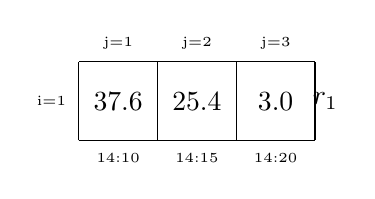
\begin{tikzpicture}
	\definecolor{mycolor}{RGB}{224,224,224}
	\definecolor{mycolor2}{RGB}{192,192,192}
	\draw[step=1cm,color=black] (0,0) grid (3,1);
	\node at (0.5,+0.5) [label={[font=\tiny,label distance=0.3cm]above:$\text{j=1}$}, label={[font=\tiny,label distance=0.1cm]left:$\text{i=1}$}, label={[font=\tiny,label distance=0.3cm]below:$\text{14:10}$}]{37.6};
	\node at (1.5,+0.5) [label={[font=\tiny,label distance=0.3cm]above:$\text{j=2}$},label={[font=\tiny,label distance=0.3cm]below:$\text{14:15}$}]{25.4};
	\node at (2.5,+0.5) [label=right:$r_1$,label={[font=\tiny,label distance=0.3cm]above:$\text{j=3}$},label={[font=\tiny,label distance=0.3cm]below:$\text{14:20}$}]{3.0};	
	\end{tikzpicture}
	\caption{Query Pattern Q(t) of length $l=3$ and $d=1$ reference time series.}
	\label{Qpatt}
\end{figure}

\begin{figure}[htbp]
	\centering
	\begin{tikzpicture}[
	scale=0.7,
	every node/.style={outer sep=0pt, transform shape, font=\scriptsize},
	every matrix/.style={cells={scale=0.7}},
	]
	
		\definecolor{myorange}{RGB}{255,178,102}
		\definecolor{myblue}{RGB}{51,153,255}
		\definecolor{myyellow}{RGB}{255,255,102}
		
		% circular array
		\xyshift{-15mm}{-100mm}{
			\matrix [ampersand replacement=\&, outer sep=0pt, matrix anchor=north] (array) {
				\node[circularptr, fill=myorange] (c1)  {37.6}; \&
				\node[circularptr, fill=myblue] (c2)  {25.4}; \&
				\node[circularptr, fill=myyellow] (c3)  {3.0}; \&
				\node[circularptr] (c4)  {13.2}; \&
				\node[circularptr] (c5)  {23.0}; \&
				\node[circularptr] (c6)  {17.1}; \&
				\node[circularptr] (c7)  {37.6}; \&
				\node[circularptr] (c8)  {18.1}; \&
				\node[circularptr] (c9)  {7.2}; \&
				\node[circularptr] (c10) {25.4}; \&
				\node[circularptr] (c11) {38.9}; \&
				\node[circularptr] (c12) {47.1}; \&
				\node[circularptr] (c13) {43.1}; \&
				\node[circularptr] (c14) {2.5};  \\
				%
				\node[circularval, fill=myorange] (left) {14:10}; \&
				\node[circularval, fill=myblue] {14:15}; \&
				\node[circularval, fill=myyellow] {14:20}; \&
				\node[circularval] {13:15}; \&
				\node[circularval] {13:20}; \&
				\node[circularval] {13:25}; \&
				\node[circularval] {13:30}; \&
				\node[circularval] {13:35}; \&
				\node[circularval] {13:40}; \&
				\node[circularval] {13:45}; \&
				\node[circularval] {13:50}; \&
				\node[circularval] {13:55}; \&
				\node[circularval] {14:00}; \&
				\node[circularval] (right){14:05};\\
			};
		}
	

	
	
	
	% root node
	\xyshift{-20mm}{0mm}{\btreeinodethree{root}{17.1}{}{}};
	
	%
	% intermediate nodes
	\xyshift{-50mm}{-15mm}{\btreeinodethree{n1}{7.2}{}{}{}}
	\xyshift{ 10mm}{-15mm}{\btreeinodethree{n2}{23.0}{37.6}{43.1}}
	%
	% connecting root to intermediate level nodes
	\foreach \x in {1,2} { \btreelink{root-\x}{n\x} }
	%
	% leaf nodes
	\xyshift{-90mm}{-30mm}{\btreelnodethree{n11}{2.5}{3.0}{}}
	\xyshift{-60mm}{-30mm}{\btreelnodethree{n12}{7.2}{13.2}{}}
	\xyshift{-30mm}{-30mm}{\btreelnodethree{n21}{17.1}{18.1}{}}
	\xyshift{ 0mm}{-30mm}{\btreelnodethree{n22}{23.0}{25.4}{}}
	\xyshift{ 30mm}{-30mm}{\btreelnodethree{n23}{37.6}{38.9}{}}
	\xyshift{ 60mm}{-30mm}{\btreelnodethree{n24}{43.1}{47.1}{}}
	%
	% connecting intermediate level to leaf nodes
	\foreach \x in {1,2}     { \btreelink{n1-\x}{n1\x} }
	\foreach \x in {1,2,3,4} { \btreelink{n2-\x}{n2\x} }
	%
	% leaf pointers
	\draw[btlink] ([yshift=+3pt] n11-c.east) -- ([yshift=+3pt] n12-a.west);
	\draw[btlink] ([yshift=-3pt] n12-a.west) -- ([yshift=-3pt] n11-c.east);
	\draw[btlink] ([yshift=+3pt] n12-c.east) -- ([yshift=+3pt] n21-a.west);
	\draw[btlink] ([yshift=-3pt] n21-a.west) -- ([yshift=-3pt] n12-c.east);
	\draw[btlink] ([yshift=+3pt] n21-c.east) -- ([yshift=+3pt] n22-a.west);
	\draw[btlink] ([yshift=-3pt] n22-a.west) -- ([yshift=-3pt] n21-c.east);
	\draw[btlink] ([yshift=+3pt] n22-c.east) -- ([yshift=+3pt] n23-a.west);
	\draw[btlink] ([yshift=-3pt] n23-a.west) -- ([yshift=-3pt] n22-c.east);
	\draw[btlink] ([yshift=+3pt] n23-c.east) -- ([yshift=+3pt] n24-a.west);
	\draw[btlink] ([yshift=-3pt] n24-a.west) -- ([yshift=-3pt] n23-c.east);
	%
	
	% circular array
	\xyshift{-40mm}{-60mm}{
		\matrix [ampersand replacement=\&, outer sep=0pt, matrix anchor=north] (array) {
			\node[circularptr] (c1)  {}; \\	
			%
			\node[circularval] (left)(right) {13:45}; \\
		};
	}
	% circular array
	\xyshift{-10mm}{-60mm}{
		\matrix [ampersand replacement=\&, outer sep=0pt, matrix anchor=north] (array) {
			\node[circularptr, fill=myblue] (c2)  {}; \\	
			%
			\node[circularval,fill=myblue] (left)(right) {14:15}; \\
		};
	}	
	
	
		% circular array
		\xyshift{20mm}{-60mm}{
			\matrix [ampersand replacement=\&, outer sep=0pt, matrix anchor=north] (array) {
				\node[circularptr] (c5)  {}; \\	
				%
				\node[circularval] (left)(right) {13:30}; \\
			};
		}
		% circular array
		\xyshift{50mm}{-60mm}{
			\matrix [ampersand replacement=\&, outer sep=0pt, matrix anchor=north] (array) {
				\node[circularptr, fill=myorange] (c6)  {}; \\	
				%
				\node[circularval,fill=myorange] (left)(right) {14:10}; \\
			};
		}	
		% draw pointers between circular array and B+ tree
		\path[btlink2] ([yshift=-2pt] c5.center)  edge[out=90,in=270] ([yshift=2pt] n23-1.center);
		% draw pointers for linked list
		\draw[btlink] ([yshift=-10pt] c5.east) -- ([yshift=-10pt] c6.west);
		\draw[btlink] ([yshift=-20pt] c6.west) -- ([yshift=-20pt] c5.east);
		
		%circular links
		\path[btlink] ([yshift=-10pt] c5.west)  edge[out=220,in=250] ([yshift=-10pt] c6.east);
		\path[btlink2] ([yshift=-20pt] c5.west)  edge[out=220,in=250] ([yshift=-20pt] c6.east);	
		
		
	
	% draw pointers between circular array and B+ tree
	\path[btlink2] ([yshift=-2pt] c1.center)  edge[out=90,in=270] ([yshift=2pt] n22-2.center);
	% draw pointers for linked list
	\draw[btlink] ([yshift=-10pt] c1.east) -- ([yshift=-10pt] c2.west);
	%\draw[btlink] ([yshift=-10pt] c2.east) -- ([yshift=-10pt] c1.east);
	\draw[btlink] ([yshift=-20pt] c2.west) -- ([yshift=-20pt] c1.east);
	
	%circular links
	\path[btlink] ([yshift=-10pt] c1.west)  edge[out=220,in=250] ([yshift=-10pt] c2.east);
	\path[btlink2] ([yshift=-20pt] c1.west)  edge[out=220,in=250] ([yshift=-20pt] c2.east);
	
	
	% list  value
	\xyshift{-90mm}{-50mm}{
		\matrix [ampersand replacement=\&, outer sep=0pt, matrix anchor=north] (array) {
			\node[circularptr] (c3)  {}; \\	
			%
			\node[circularval] (left)(right) {14:05}; \\
		};
	}
	
	% draw pointers between list value and B+ tree
	\path[btlink2] ([yshift=-2pt] c3.center)  edge[out=90,in=270] ([yshift=2pt] n11-1.center);
	
	%circular links
	\path[btlink] ([yshift=-16pt] c3.west)  edge[out=-1500,in=-60] ([yshift=-16pt] c3.east);
	\path[btlink2] ([yshift=-24pt] c3.west)  edge[out=-1500,in=-60] ([yshift=-24pt] c3.east);
	
	
	% list  value
	\xyshift{-70mm}{-50mm}{
		\matrix [ampersand replacement=\&, outer sep=0pt, matrix anchor=north] (array) {
			\node[circularptr,fill=myyellow] (c4)  {}; \\	
			%
			\draw node [black,midway,yshift=-0.9cm] {leftPos$^-$ = rightPos$^+$};
			\node[circularval, fill=myyellow] (left)(right) {14:20}; \\
		};
	}
	
	% draw pointers between list value and B+ tree
	\path[btlink2] ([yshift=-2pt] c4.center)  edge[out=90,in=270] ([yshift=2pt] n11-2.center);
	
	%circular links
	\path[btlink] ([yshift=-16pt] c4.west)  edge[out=-1500,in=-60] ([yshift=-16pt] c4.east);
	\path[btlink2] ([yshift=-24pt] c4.west)  edge[out=-1500,in=-60] ([yshift=-24pt] c4.east);
	
	\foreach \x in
	{n12-1,n12-2,n21-1,n21-2,n22-1, n23-2, n23-3, n24-1,n24-2}
	{ \path[<-] ([yshift=-15pt] \x.center) edge ([yshift=2pt] \x.center); }
	%
	

	\end{tikzpicture}
	\vspace{2mm}
	\caption{The circular array and the $B^+$tree for time series $r_1$ after initialization.}
	\label{fig:initialize}
\end{figure}





\begin{algorithm}[H]
	\IncMargin{1em}
	\SetAlgoLined
	\DontPrintSemicolon
	\KwIn{Tree $tree$, the node $node$ and its neighbor $neighbor$, the neighborIndex $nIndex$, the $kIndex$ and the the key $kPrime$}
	\KwOut{The keys in the node and its neighbor, as well as the parents keys are redestributed}
	

		    neighboorhood.key $\leftarrow$ measurement.value\;
		    neighboorhood.j $\leftarrow$ j\;
		    neighboorhood.patternLength $\leftarrow$ l\;
		    
		    \BlankLine
		    leafNode $\leftarrow$ findLeaf(tree, measurement.value)\;
		    pointerIndex $\leftarrow$ getInsertionIndex(leafNode, measurement.value)\;
		    elementOnThatKey $\leftarrow$ leafNode.pointers[pointerIndex]\;
		    \BlankLine
		    //Upper Bound: The value is at most patternLength away form first list value\;
		    maxSteps $\leftarrow$ patternLength\;
		    \While{elementOnThatKey.timestamp $\neq$ measurement.timestamp \&\& maxSteps $\neq$ 0}{
		    	//go from newest value back towards oldest\;
		    	elementOnThatKey $\leftarrow$ elementOnThatKey.prev\;
		    	maxSteps--\;
		    }

		    neighboorhood.leftPos $\leftarrow$ set position to elementOnThatKey\;
		    neighboorhood.rightPos $\leftarrow$ set position to elementOnThatKey\;
		    \BlankLine
		    \Return neighboorhood;
	
	
	

	\caption{NewNeighborhood$(t,v,j,l)$}	\label{initializeNeighborhood}
\end{algorithm}



\subsection{Sorted Access: Grow Neighborhood}
After the initialization of the $l \times d$ neighborhoods the $k$ non-overlapping patterns are calculated. Thus, the sortedAccess$(v, T)$ operation is executed until the $k$ patterns that contain the most similar values to $q_{ij}$ are retrieved.\\
The sortedAccess$(v, T)$ operation searches the time point for the next most similar value to a query pattern cell $q_{ij}$ of the query pattern $Q(t)$. The neighborhood $N(q_{ij})$ is expanded until such a value is retrieved. Some time points may have to be skipped because the time point anchored a pattern previously. The next unseen most similar value to $q_{ij}$ is either at position $t^-$ or $t^+$, which represent the time points to the direct left or right of leftPos$^-$ and rightPos$^+$. If the $t^-$ is more or equally similar to $q_{ij}$ than $t^+$, the leftPos$^-$ is decremented and $t=t^-$. If $t^+$ is more similar $t=t^+$.

\begin{example}
Figure \ref{fig:increase} shows how the neighborhood $N(q_{12})$ is expanded. We assume that the other neighborhoods $N(q_{11})$ and $N(q_{13})$ has not been initialized yet. 
Hence, there are no additional time points anchored for a pattern previously and the timeset $T$ is initially empty. If the Neighbor$(v,T)$ is executed 3 times the resulting neighborhood will look as follows:  
\end{example}

\begin{figure}[htbp]
	\centering
	\begin{tikzpicture}[
	scale=0.7,
	every node/.style={outer sep=0pt, transform shape, font=\scriptsize},
	every matrix/.style={cells={scale=0.7}},
	]
	
	\definecolor{myorange}{RGB}{255,178,102}
	\definecolor{myblue}{RGB}{51,153,255}
	\definecolor{myyellow}{RGB}{255,255,102}

	% leaf nodes
	\xyshift{-90mm}{-30mm}{\btreelnodethree{n11}{2.5}{3.0}{}}
	\xyshift{-60mm}{-30mm}{\btreelnodethree{n12}{7.2}{13.2}{}}
	\xyshift{-30mm}{-30mm}{\btreelnodethree{n21}{17.1}{18.1}{}}
	\xyshift{ 0mm}{-30mm}{\btreelnodethree{n22}{23.0}{25.4}{}}
	\xyshift{ 30mm}{-30mm}{\btreelnodethree{n23}{37.6}{38.9}{}}
	\xyshift{ 60mm}{-30mm}{\btreelnodethree{n24}{43.1}{47.1}{}}
	%
	% leaf pointers
	\draw[btlink] ([yshift=+3pt] n11-c.east) -- ([yshift=+3pt] n12-a.west);
	\draw[btlink] ([yshift=-3pt] n12-a.west) -- ([yshift=-3pt] n11-c.east);
	\draw[btlink] ([yshift=+3pt] n12-c.east) -- ([yshift=+3pt] n21-a.west);
	\draw[btlink] ([yshift=-3pt] n21-a.west) -- ([yshift=-3pt] n12-c.east);
	\draw[btlink] ([yshift=+3pt] n21-c.east) -- ([yshift=+3pt] n22-a.west);
	\draw[btlink] ([yshift=-3pt] n22-a.west) -- ([yshift=-3pt] n21-c.east);
	\draw[btlink] ([yshift=+3pt] n22-c.east) -- ([yshift=+3pt] n23-a.west);
	\draw[btlink] ([yshift=-3pt] n23-a.west) -- ([yshift=-3pt] n22-c.east);
	\draw[btlink] ([yshift=+3pt] n23-c.east) -- ([yshift=+3pt] n24-a.west);
	\draw[btlink] ([yshift=-3pt] n24-a.west) -- ([yshift=-3pt] n23-c.east);
	%
	
	% circular array
	\xyshift{-40mm}{-60mm}{
		\matrix [ampersand replacement=\&, outer sep=0pt, matrix anchor=north] (array) {
			\node[circularptr] (c1)  {}; \\	
			%
			\node[circularval] (left)(right) {13:45}; \\
		};
	}
	% circular array
	\xyshift{-10mm}{-60mm}{
		\matrix [ampersand replacement=\&, outer sep=0pt, matrix anchor=north] (array) {
			\node[circularptr, fill=myblue] (c2)  {}; \\	
			%
			\node[circularval,fill=myblue] (left)(right) {14:15}; \\
		};
	}	
	
	
	% circular array
	\xyshift{20mm}{-60mm}{
		\matrix [ampersand replacement=\&, outer sep=0pt, matrix anchor=north] (array) {
			\node[circularptr] (c5)  {}; \\	
			%
			\node[circularval] (left)(right) {13:30}; \\
		};
	}
	% circular array
	\xyshift{50mm}{-60mm}{
		\matrix [ampersand replacement=\&, outer sep=0pt, matrix anchor=north] (array) {
			\node[circularptr] (c6)  {}; \\	
			%
			\node[circularval] (left)(right) {14:10}; \\
		};
	}	
	% draw pointers between circular array and B+ tree
	\path[btlink2] ([yshift=-2pt] c5.center)  edge[out=90,in=270] ([yshift=2pt] n23-1.center);
	% draw pointers for linked list
	\draw[btlink] ([yshift=-10pt] c5.east) -- ([yshift=-10pt] c6.west);
	\draw[btlink] ([yshift=-20pt] c6.west) -- ([yshift=-20pt] c5.east);
	
	%circular links
	\path[btlink] ([yshift=-10pt] c5.west)  edge[out=220,in=250] ([yshift=-10pt] c6.east);
	\path[btlink2] ([yshift=-20pt] c5.west)  edge[out=220,in=250] ([yshift=-20pt] c6.east);	
	
	
	
	% draw pointers between circular array and B+ tree
	\path[btlink2] ([yshift=-2pt] c1.center)  edge[out=90,in=270] ([yshift=2pt] n22-2.center);
	% draw pointers for linked list
	\draw[btlink] ([yshift=-10pt] c1.east) -- ([yshift=-10pt] c2.west);
	%\draw[btlink] ([yshift=-10pt] c2.east) -- ([yshift=-10pt] c1.east);
	\draw[btlink] ([yshift=-20pt] c2.west) -- ([yshift=-20pt] c1.east);
	
	%circular links
	\path[btlink] ([yshift=-10pt] c1.west)  edge[out=220,in=250] ([yshift=-10pt] c2.east);
	\path[btlink2] ([yshift=-20pt] c1.west)  edge[out=220,in=250] ([yshift=-20pt] c2.east);


	

	
	\foreach \x in
	{n11-1,n11-2,n12-1,n12-2,n21-1,n21-2,n22-1, n23-2, n23-3, n24-1,n24-2}
	{ \path[<-] ([yshift=-15pt] \x.center) edge ([yshift=2pt] \x.center); }
	%
	
	
	%second
	
	
	
		% leaf nodes
		\xyshift{-90mm}{-90mm}{\btreelnodethree{xn11}{2.5}{3.0}{}}
		\xyshift{-60mm}{-90mm}{\btreelnodethree{xn12}{7.2}{13.2}{}}
		\xyshift{-30mm}{-90mm}{\btreelnodethree{xn21}{17.1}{18.1}{}}
		\xyshift{ 0mm}{-90mm}{\btreelnodethree{xn22}{23.0}{25.4}{}}
		\xyshift{ 30mm}{-90mm}{\btreelnodethree{xn23}{37.6}{38.9}{}}
		\xyshift{ 60mm}{-90mm}{\btreelnodethree{xn24}{43.1}{47.1}{}}
		%
		% leaf pointers
		\draw[btlink] ([yshift=+3pt] xn11-c.east) -- ([yshift=+3pt] xn12-a.west);
		\draw[btlink] ([yshift=-3pt] xn12-a.west) -- ([yshift=-3pt] xn11-c.east);
		\draw[btlink] ([yshift=+3pt] xn12-c.east) -- ([yshift=+3pt] xn21-a.west);
		\draw[btlink] ([yshift=-3pt] xn21-a.west) -- ([yshift=-3pt] xn12-c.east);
		\draw[btlink] ([yshift=+3pt] xn21-c.east) -- ([yshift=+3pt] xn22-a.west);
		\draw[btlink] ([yshift=-3pt] xn22-a.west) -- ([yshift=-3pt] xn21-c.east);
		\draw[btlink] ([yshift=+3pt] xn22-c.east) -- ([yshift=+3pt] xn23-a.west);
		\draw[btlink] ([yshift=-3pt] xn23-a.west) -- ([yshift=-3pt] xn22-c.east);
		\draw[btlink] ([yshift=+3pt]xn23-c.east) -- ([yshift=+3pt] xn24-a.west);
		\draw[btlink] ([yshift=-3pt] xn24-a.west) -- ([yshift=-3pt] xn23-c.east);
		%
		
		% circular array
		\xyshift{-40mm}{-120mm}{
			\matrix [ampersand replacement=\&, outer sep=0pt, matrix anchor=north] (array) {
				\node[circularptr,fill=myblue] (xc1)  {}; \\	
				%
				\node[circularval,fill=myblue] (left)(right) {13:45}; \\
			};
		}
		% circular array
		\xyshift{-10mm}{-120mm}{
			\matrix [ampersand replacement=\&, outer sep=0pt, matrix anchor=north] (array) {
				\node[circularptr, fill=myblue] (xc2)  {}; \\	
				%
				\node[circularval,fill=myblue] (left)(right) {14:15}; \\
			};
		}	
		
		
		% circular array
		\xyshift{20mm}{-120mm}{
			\matrix [ampersand replacement=\&, outer sep=0pt, matrix anchor=north] (array) {
				\node[circularptr] (xc5)  {}; \\	
				%
				\node[circularval] (left)(right) {13:30}; \\
			};
		}
		% circular array
		\xyshift{50mm}{-120mm}{
			\matrix [ampersand replacement=\&, outer sep=0pt, matrix anchor=north] (array) {
				\node[circularptr] (xc6)  {}; \\	
				%
				\node[circularval] (left)(right) {14:10}; \\
			};
		}	
		% draw pointers between circular array and B+ tree
		\path[btlink2] ([yshift=-2pt] xc5.center)  edge[out=90,in=270] ([yshift=2pt] xn23-1.center);
		% draw pointers for linked list
		\draw[btlink] ([yshift=-10pt] xc5.east) -- ([yshift=-10pt] xc6.west);
		\draw[btlink] ([yshift=-20pt] xc6.west) -- ([yshift=-20pt] xc5.east);
		
		%circular links
		\path[btlink] ([yshift=-10pt] xc5.west)  edge[out=220,in=250] ([yshift=-10pt] xc6.east);
		\path[btlink2] ([yshift=-20pt] xc5.west)  edge[out=220,in=250] ([yshift=-20pt] xc6.east);	
		
		
		
		% draw pointers between circular array and B+ tree
		\path[btlink2] ([yshift=-2pt] xc1.center)  edge[out=90,in=270] ([yshift=2pt] xn22-2.center);
		% draw pointers for linked list
		\draw[btlink] ([yshift=-10pt] xc1.east) -- ([yshift=-10pt] xc2.west);
		%\draw[btlink] ([yshift=-10pt] c2.east) -- ([yshift=-10pt] c1.east);
		\draw[btlink] ([yshift=-20pt] xc2.west) -- ([yshift=-20pt] xc1.east);
		
		%circular links
		\path[btlink] ([yshift=-10pt] xc1.west)  edge[out=220,in=250] ([yshift=-10pt] xc2.east);
		\path[btlink2] ([yshift=-20pt] xc1.west)  edge[out=220,in=250] ([yshift=-20pt] xc2.east);
		
		
			% list  value
			\xyshift{-60mm}{-120mm}{
				\matrix [ampersand replacement=\&, outer sep=0pt, matrix anchor=north] (array) {
					\node[circularptr,fill=myblue] (c3)  {}; \\	
					%
					\node[circularval,fill=myblue] (left)(right) {13:20}; \\
				};
			}
			
			% draw pointers between list value and B+ tree
			\path[btlink2] ([yshift=-2pt] c3.center)  edge[out=90,in=270] ([yshift=2pt] xn22-1.center);
			
			%circular links
			\path[btlink] ([yshift=-16pt] c3.west)  edge[out=-1500,in=-60] ([yshift=-16pt] c3.east);
			\path[btlink2] ([yshift=-24pt] c3.west)  edge[out=-1500,in=-60] ([yshift=-24pt] c3.east);
		
				
				% list  value
				\xyshift{-80mm}{-120mm}{
					\matrix [ampersand replacement=\&, outer sep=0pt, matrix anchor=north] (array) {
						\node[circularptr,fill=myblue] (c7)  {}; \\	
						%
						\node[circularval,fill=myblue] (left)(right) {13:35}; \\
					};
				}
				
				% draw pointers between list value and B+ tree
				\path[btlink2] ([yshift=-2pt] c7.center)  edge[out=90,in=270] ([yshift=2pt] xn21-2.center);
				
				%circular links
				\path[btlink] ([yshift=-16pt] c7.west)  edge[out=-1500,in=-60] ([yshift=-16pt] c7.east);
				\path[btlink2] ([yshift=-24pt] c7.west)  edge[out=-1500,in=-60] ([yshift=-24pt] c7.east);
				
		
		
		\foreach \x in
		{xn11-1,xn11-2,xn12-1,xn12-2,xn21-1, xn23-2, xn23-3, xn24-1,xn24-2}
		{ \path[<-] ([yshift=-15pt] \x.center) edge ([yshift=2pt] \x.center); }
		%
		
		
	
	
	
	\end{tikzpicture}
	\vspace{2mm}
	\caption{Status of $N(q_{1,2})$ after growing 3 times.}
	\label{fig:increase}
\end{figure}




\begin{algorithm}[H]
	\IncMargin{1em}
	\SetAlgoLined
	\DontPrintSemicolon
	\KwIn{Query pattern value $v$ and the set of visited time points $T$ and the neighborhood itself $self$}
	\KwOut{Time point of the next most similar value to $v$}
	

		    leftPos$^-$ $\leftarrow$ self.leftPos\;
		    rightPos$^+$ $\leftarrow$ self.rightPos\;


		    \While{$t^-$ $\neq$ NIL and TimeSetContains($t^-$ $-(j + l)$)}{
		    	
			    leftPos$^-$ $\leftarrow$ leftPos$^-$ $- 1$\;
		    }
		    
		    \While{$t^-$ $\neq$ NIL and TimeSetContains($t^-$ $-(j + l)$)}{
		      	
		     	rightPos$^+$ $\leftarrow$ rightPos$^+$ $+ 1$\;
		    }
		    
		   \uIf{$t^-$ $\neq$ NIL and  $t^+$ $\neq$ NIL }{
			   	\eIf{$|r_{i}(t^-)$ - self.key$|$ $\leq$ $|r_{i}(t^+)$ - self.key$|$}{
		   		
			   		leftPos$^-\leftarrow$ leftPos$^- - 1$\; $t$ $\leftarrow$ $t^-$\;
		 		
			   	}
			   	{
			   		rightPos$^+\leftarrow$ rightPos$^+ + 1$\; $t$ $\leftarrow$ $t^+$\;
			   	}
		   	}
		   	\uElseIf{$t^-$ $\neq$ NIL}{
		   		
		   		leftPos$^-\leftarrow$ leftPos$^- - 1$\; $t$ $\leftarrow$ $t^-$\;
		   	}
		   	\uElseIf{$t^+$ $\neq$ NIL}{
		   		rightPos$^+\leftarrow$ rightPos$^+ + 1$\; $t$ $\leftarrow$ $t^+$\;
		   		
		   	}
		   	\Else{
		   		\Return NIL\; 	
		   	}
		   
	
		    \Return t\;
	
	
	

	\caption{SortedAccess$(v, T)$}	\label{NeighborhoodGrow}
\end{algorithm}




\chapter{Complexity Analysis}
\label{Complexity}
This analysis refers to a single time series $s$ for which a $B^+$tree and a circular array are maintained and the complexity calculations are valid for our context, e.g. the linked list elements are traversed at most $l$ times. 
\newtheorem{mydef}{Lemma}

\subsection{Runtime Complexity}

\paragraph{Circular, Doubly Linked List}
\begin{mydef}
	The insertion of a new time point to a linked list needs $O(1)$ time.
\end{mydef}
\begin{proof}
	For each new value produced by a time series $s$ a linked list in the $B^+$tree is expanded. Since the new value is always inserted at the tail position it needs $O(1)$.
\end{proof}
\begin{mydef}
	The deletion of a time point from a linked list needs $O(1)$ time.
\end{mydef}
\begin{proof}
	For each deletion in a $B^+$tree a time point needs to be removed from a linked list. Since the oldest value is always at the head position, the deletion needs $O(1)$.
\end{proof}
\begin{mydef}
	The search of a specific time point in a linked list if newNeighborhood$(t,v,j,l)$ is executed takes at most $O(l)$ time.
\end{mydef}
\begin{proof}
	A time series $s$ in a pattern $P(t)$ initializes $l$ neighborhoods. Hence in the worst case, if the $l$ newest measurements in the circular array of $s$ have the same value and thus are stored in the same linked list in the $B^+$tree, $l$ list elements have to be traversed to find the specific measurement time point. 
\end{proof}

\subsubsection{Circular Array Operations}
\begin{mydef}
	The update of the circular array takes $O(1)$ time.
\end{mydef}
\begin{proof}
	The next update position in a circular array is computet in $O(1)$ time, hence the update takes $O(1)$ time. 
\end{proof}
\begin{mydef}
	The random access of a time point $t$ takes $O(1)$ time.
\end{mydef}
\begin{proof}
	The random access algorithm needs to calculate the position for the time point $t$. Since the position can be directly calculated the calculation is done in $O(1)$.
\end{proof}

\subsubsection{$B^+$tree Operations}

Normally, the complexity of operations on $B^+$trees is dependent on the 
required I/O operations since I/O operations are expensive. The speed of operations on $B^+$trees makes it a frequently used index structure in database implementations. But since we do not have I/O operations the complexity of our implementation is also dependent on the tree node size which usually is neglected.


\begin{mydef}
	The search of a measurement in the $B^+$tree takes at most $O(l + (\log_{n}(|W|) \times n))$ time.
	\label{def1}
\end{mydef}
\begin{proof}
	To search the insertion and deletion position in a $B^+$tree takes $O(\log_{n}(|W|) \times n)$. For the sortedAccess$(v,T)$ operation the pattern length $l$ provides an upper bound for the maximum required value lookups in a doubly, linked list.\\ The nodes are traversed, recursively and downwards from the root of the tree. Therefore, the problem of size $|W|$ is divided by the tree order $n$. This leads to $log_n(|W|)$ complexity, where $|W|$ is the maximum number of keys in the tree, at the same time the size of the circular array, and $n$ is the order of the tree, representing the maximum number of pointers in a node. \\The time taken to find the appropriate pointer index $i$ in the $FindLeaf$ operation is at most $O(n)$. Hence, the total complexity to find a leaf key is $O((\log_{n}(|W|) \times n))$. 
\end{proof}

\begin{mydef}
	The insertion of a measurement to the $B^+$tree takes $O(\log_{n}(|W|) \times n)$ time.
\end{mydef}
\begin{proof}
	In the worst case for an insertion is proportional to $\log_{n}(|W|)$, where $n$ is the maximum number of pointers in a node. The number of keys in leaf nodes is at most $|W|$. If there are no duplicate values in the circular array. In our case the insertion point of a new measurement to a doubly, linked list is always found in $O(1)$, duplicates have no influence to the complexity of an insertion.  
\end{proof}
\begin{mydef}
	The deletion of a measurement from the $B^+$tree takes $O(\log_{n}(|W|) \times n)$ time.
\end{mydef}
\begin{proof}
	 If there are no duplicate values the number of leaf keys is the size of the time window $|W|$. Since the deletion point of a new measurement from a doubly, linked list is always found in $O(1)$, duplicates as well have no influence to the complexity of a deletion. 
\end{proof}


\subsubsection{Neighborhood Operations}
\begin{mydef}
	The initialization of a neighborhood in time series $s$ takes $O(l+(\log_{n}(|W|) \times n)))$ time.
\end{mydef}
\begin{proof}
	The initialization of the neighborhood needs to search a specific measurement in the $B^+$tree. Hence the complexity is equal to the search operation in a $B^+$tree defined in \ref{def1}. The pattern length gives an upper bound to the maximum required value lookups in a doubly, linked list.
\end{proof}

\begin{mydef}
	The sortedAccess$(v,T)$ takes at most $O(|T|)$ time.
\end{mydef}
\begin{proof}
	If the time set contains $|T|$ time points and since at most $|T|$ time points have to be skipped the sortedAccess$(v,T)$ takes at most at most $O(|T|)$ time. 
\end{proof}

\subsection{Space Complexity}
The $B^+$tree structure imposes performance overhead on insertion
and deletion, and adds space overhead. But the cost of reorganization of the measurements is avoided. Furthermore,
since nodes may be as much as half empty (if they have the minimum
number of children), there is some wasted space. This space overhead, is
acceptable given the performance benefits of the $B^+$tree structure.
\begin{mydef}
	The space complexity of a circular array is $O(|W|)$.
\end{mydef}
\begin{proof}
	Every circular array for a time series $s$ has a size |W|. Hence the space complexity of one circular array is $O(|W|)$.
\end{proof}

\begin{mydef}
	The space complexity of a $B^+$tree is $O(|W|)$. 
\end{mydef}
\begin{proof}
	Each measurement is stored once in the tree. Hence, the tree may have at most $|W|$ nodes.  
\end{proof}



\chapter{Experimental Evaluation}
\label{sec:Experimental}
This chapter describes our experimental setup and results. We evaluated the runtime of the $shift$ algorithm with different values for the tree node size $n-1$ and parameter $W$. 


\section{Setup}
In the experiments we construct a data set with measurement values with a time span of 100 years between the newest and the oldest value. We use one time series $r$, thus $d=1$. The interval between two values is set to $3$ minutes. Since 20 measurements arrive per hour the data set contains in total 17'520'000 measurements in 100 years (100$\times$365$\times$24$\times$20). Assuming every of these 100 years has 365 days. We assume the data set contains values between 0 and 10000 and duplicates are possible. The values are random but always between these bounds. 

\section{Runtime}


\paragraph{Tree Node Size.}
The size of a node determines the number of values it can hold. We set the window size $|W|$ to 3 years for this experiment and show the effect of an increasing tree node size. 

\begin{table}[H]
	\centering
	\begin{tikzpicture}
	\begin{axis}[ width=0.8\textwidth,
	height=0.5\textwidth,
	width=\linewidth, % Scale the plot to \linewidth
	grid=major, % Display a grid
	grid style={dashed,gray!50}, % Set the style
	xlabel=Node size, % Set the labels
	ylabel=ms
	={at={(2,-5)},anchor=north}, % Put the legend below the plot
	x label style={at={(axis description cs:0.5,-0.03)},anchor=north},
	y label style={at={(axis description cs:-0.01,.5)},anchor=south},
	x tick label style={rotate=90,anchor=east} % Display labels sideways
	]
	\addplot 
	% add a plot from table; you select the columns by using the actual name in
	% the .csv file (on top)
	table[x=Nodesize,y=ms,col sep=comma] {data1.csv}; 
	\legend{Plot}
	\end{axis}
	\end{tikzpicture}
	\caption{Shift operation with increasing values for $n-1$.}
\end{table}



\paragraph{Window Size.}
The window size $|W|$ determines the number of measurements stored in the circular array and the $B^+tree$. We show the effect of an increasing window size to the running time of the $shift$ operation. The window size is between 60 days, hence 28800 measurements (60$\times$24$\times$20) and 3 years, 525600 measurements (3$\times$365$\times$24$\times$20). The tree node size is set to 40. 

\begin{table}[H]
\begin{tikzpicture}
\begin{axis}[ width=0.8\textwidth,
height=0.5\textwidth,
width=\linewidth, % Scale the plot to \linewidth
grid=major, % Display a grid
grid style={dashed,gray!50}, % Set the style
xlabel=|W|, % Set the labels
ylabel=ms
={at={(2,-5)},anchor=north}, % Put the legend below the plot
x label style={at={(axis description cs:0.5,-0.03)},anchor=north},
y label style={at={(axis description cs:-0.01,.5)},anchor=south},
x tick label style={rotate=90,anchor=east} % Display labels sideways
]
\addplot 
% add a plot from table; you select the columns by using the actual name in
% the .csv file (on top)
table[x=W,y=ms,col sep=comma] {resultsw.csv}; 
\legend{Plot}
\end{axis}
\end{tikzpicture}
	\caption{Shift operation with increasing values for $|W|$.}
\end{table}

\chapter{Summary and Conclusion}
\label{sec:Summary}
We studied the requirements for keeping a portion of a streaming time series in main memory and simultaneously provide efficient access possibilities to the measurements in a time series. The system we presented uses two different data structures to achieve efficient access operations. Random access is efficiently performed on a circular array and sorted access is efficiently performed on a $B^+$tree with leaves linked in both directions, thus, to the respective successor and predecessor. \\Furthermore, the system can handle duplicate values with a simple but powerful circular, doubly linked list. The duplicate handling is not only simple to implement but also effective in terms of update velocity. Moreover, retrieving a specific value in the linked list has an upper bound and therefore is efficiently performed in most cases. 






\begin{thebibliography}{99}
	\bibliographystyle{alpha}
	
	\bibitem{BScT} K. Wellenzohn, M. Böhlen, A. Dignös, J. Gamper, and H. Mitterer: \emph{Continuous imputation of missing values in highly correlated streams of time series data}; Unpublished, 2016.
	
	\bibitem{DatabaseSystemC} Abraham Silberschatz, Henry F. Korth, S. Sudarshan: \emph{Database System Concepts}; ISBN 978-0-07-352332-3, 2011 by The McGraw-Hill Companies, Inc.
	
	\bibitem{LinkedListBook} Thomas H. Cormen, Charles E. Leiserson, Ronald L.Rivest, Clifford Stein: \emph{Introduction to Algorithms}; Massachusetts Institute of Technology, Massachusetts, USA, 2009. 
	
	
\end{thebibliography}




\appendix%*{Appendix}

\appendixpage


\addappheadtotoc
\chapter{Algorithms}



\section{Deletion}

\begin{algorithm}[H]
	\IncMargin{1em}
	\SetAlgoLined
	\DontPrintSemicolon
	\KwIn{Tree $tree$}
	\KwOut{The $tree$ with an adjusted root node}
	
	//enough keys in the root\;
	\If{0 < tree.root.numOfKeys}{
		\Return\; 	
	}
	//if the root has a child, promote the first (only) child as the new root\;
	\eIf{root is not a leaf}{
		newRoot $\leftarrow$ tree.root.pointers[0]\;
		newRoot.parent $\leftarrow$ NIL\;
	}
	{
		newRoot $\leftarrow$ NIL\;
	}
	
	tree.root $\leftarrow$ newRoot\;
	
	\caption{AdjustTheRoot$(tree)$}	\label{adjustTheRoot}
\end{algorithm}



\begin{algorithm}[H]
	\IncMargin{1em}
	\SetAlgoLined
	\DontPrintSemicolon
	\KwIn{Tree $tree$, the $node$ and its neighbor $neighbor$, the neighborIndex $nIndex$ and the key $kPrime$}
	\KwOut{$node$ and its $neighbor$ are merged to one node}
	
	//Swap neighbor with node if node is on the extreme left and neighbor is to its right\;
	\If{nIndex = -1}{
		swap neighbor with node\;
	}
	neighborInsertionIndex $\leftarrow$ neighbor.numOfKeys\;
	
	\eIf{node is no leaf}{
		neighbor.keys[neighborInsertionIndex] $\leftarrow$ kPrime\;
		neighbor.numOfKeys++\;
		decreasingIndex $\leftarrow$ 0\;
		numOfKeysBefore $\leftarrow$ node.numOfKeys\;
		\For{i $\leftarrow$ neighborInsertionIndex + 1, j $\leftarrow$ 0; j < node.numOfKeys}{
			\BlankLine
			neighbor.keys[i] $\leftarrow$ node.keys[j]\;
			neighbor.pointers[i] $\leftarrow$ node.pointers[j]\;
			neighbor.numOfKeys++\;
			decreasingIndex++, i++, j++\;
		}
		node.numOfKeys $\leftarrow$ numOfKeysBefore - decreasingIndex\;
		neighbor.pointers[i] $\leftarrow$ node.pointers[j]\;
		\BlankLine
		//All children must now point up to the same parent\;
		\For{i $\leftarrow$ 0; i < neighbor.numOfKeys + 1; i++}{
			tmp $\leftarrow$ neighbor.pointers[i]\;
			tmp.parent $\leftarrow$ neighbor\;
		}
		
	}
	{
		// a leaf, append the keys and pointers of the node to the neighbor\;
		//Set the neighbor's last pointer to point to what had been the node's right neighbor\;
		
		\For{i $\leftarrow$ neighborInsertionIndex, j $\leftarrow$ 0; j < node.numOfKeys}{
			neighbor.keys[i] $\leftarrow$ node.keys[j]\;
			neighbor.pointers[i] = node.pointers[j]\;
			neighbor.numOfKeys++, i++, j++\;
		}
		
		relink leaves\;
	}
	deleteEntry(tree, node.parent, kPrime, node)\;
	
	
	
	\caption{MergeNodes$(tree, node, neighbor, nIndex, kPrime)$}	\label{MergeNodes}
\end{algorithm}
%Merge

\begin{algorithm}[H]
	\IncMargin{1em}
	\SetAlgoLined
	\DontPrintSemicolon
	\KwIn{Tree $tree$, the node $node$ and its neighbor $neighbor$, the neighborIndex $nIndex$, the $kIndex$ and the the key $kPrime$}
	\KwOut{The keys in the $node$ and its $neighbor$, as well as the $parents$ keys are redestributed}
	
	
	//node has neighbor to the left side\;
	\eIf{nIndex != -1}{
		//Pull neighbor's last key-pointer pair\; over from the neighbor's right end to n\;
		\eIf{node is not a leaf}{
			m $\leftarrow$ neighbor.pointers[neighbor.numOfKeys]\;
			insert neighbor.pointers[m] and $kPrime$ to first position in node and shift other pointers and values right\;
			remove neighbor.key[m-1], neighbor.pointers[m] from neighbor\;
			replace $kPrime$ in node.parent by neighbor.keys[m-1]\;}
		{
			//last value pointer pair in the node\;
			m $\leftarrow$ neighbor.pointers[neighbor.numOfKeys -1]\;
			insert neighbor.pointers[m] and neighbor.keys[m] to first position in node and shift other pointers and values right\;
			remove neighbor.key[m], neighbor.pointers[m] from neighbor\;
			replace $kPrime$ in node.parent by node.keys[0]\;
		}
		
	}	
	{
		//node is leftmost child. Take a key-pointer pair from the neighbor to the right\;
		//Move the neighbor's leftmost key-pointer pair to n's rightmost position\;
		\eIf{node is not a leaf}{
			node.keys[node.numOfKeys] $\leftarrow$ $kPrime$\;
			node.pointers[node.numOfKeys +1] $\leftarrow$ neighbor.pointers[0]\;
			replace $kPrime$ in node.parent by neighbor.keys[0]\;
			remove neighbor.keys[0], neighbor.pointers[0] from neighbor\;}
		{
			node.keys[node.numOfKeys] $\leftarrow$ neighbor.keys[0]\;
			node.pointers[node.numOfKeys +1] $\leftarrow$ neighbor.pointers[0]\;
			node.parent.keys[kIndex] = neighbor.keys[1]\;
			remove neighbor.keys[0], neighbor.pointers[0] from neighbor\;
		}
	}
	
	
	\caption{Redistribute$(tree, node, neighbor, nIndex, kIndex, kPrime)$}	\label{Redistribute}
\end{algorithm}
%Redistribute

\section{Insertion}

\begin{algorithm}[H]
	\IncMargin{1em}
	\SetAlgoLined
	\DontPrintSemicolon
	\KwIn{Tree $tree$, the insertion node $leaf$, the time point $t$ and the value $v$}
	\KwOut{The leaf is split into two leaves}
	
	
	
	insertPoint $\leftarrow$ 0\;
	nrOfTempKeys $\leftarrow$ 0\;
	insertPoint $\leftarrow$ getInsertPoint(tree, leaf, v)\;
	
	//fills the keys and pointers\;
	\For{i $\leftarrow$ 0, j $\leftarrow$ 0; i < oldNode.numOfKeys;} {
		
		\If{j = insertPoint}{
			j++\;
		}
		tempKeys[j] $\leftarrow$ oldNode.keys[i]\;
		tempPointers[j] $\leftarrow$ oldNode.pointers[i]\;
		nrOfTempKeys++, i++, j++\;
	}
	
	//enter the record to the right position\;
	tempKeys[insertPoint] $\leftarrow$ v\;
	
	newList $\leftarrow$ create list and insert $t$\;
	tempPointers[insertPoint] $\leftarrow$ newList\;
	nrOfTempKeys++\;
	
	newNode.numOfKeys $\leftarrow$ 0\;
	oldNode.numOfKeys $\leftarrow$ 0\;
	\BlankLine
	//calculate splitpoint by $\ceil{n/2}$\;
	split = getSplitPoint(tree.nodeSize)\;
	
	//fill first leaf\;
	\For{i $\leftarrow$ 0; i < split} {
		oldNode.keys[i] $\leftarrow$ tempKeys[i]\;
		oldNode.pointers[i] $\leftarrow$ tempPointers[i]\;
		oldNode->numOfKeys++, i++\;
	}
	
	
	//fill second leaf\;
	\For{j $\leftarrow$ 0, i $\leftarrow$ split; i < nrOfTempKeys;} {
		newNode.keys[j] $\leftarrow$ tempKeys[i]\;
		newNode.pointers[j] $\leftarrow$ tempPointers[i]\;
		newNode->numOfKeys++, i++, j++\;
	}
	
	link leaves\;
	newNode.parent $\leftarrow$ oldNode.parent\;
	
	keyForParent $\leftarrow$ newNode.keys[0]\;
	
	insertIntoParent(tree, oldNode, keyForParent, newNode)\;
	
	
	
	
	\caption{SplitLeaves$(tree, leaf, t, v)$}	\label{SplitLeaves}
\end{algorithm}

\begin{algorithm}[H]
	\IncMargin{1em}
	\SetAlgoLined
	\DontPrintSemicolon
	\KwIn{Tree $tree$, the node $oldInnderNode$ and the child node $childNode$, the index $index$ and in addition the $key$}
	\KwOut{The inner node is split into two nodes}
	
	
	nrOfTempKeys $\leftarrow$ 0, x $\leftarrow$ 0\;
	
	\For{i $\leftarrow$ 0, j $\leftarrow$ 0; i < oldNode.numOfKeys;} {
		\If{j = index}{	j++
		}
		tempKeys[j] $\leftarrow$ oldInnerNode.keys[i], nrOfTempKeys++, i++, j++\;
		
	}
	
	\For{ i $\leftarrow$ 0, j $\leftarrow$ 0; i < oldInnerNode.numOfKeys + 1;} {
		\If{j = index + 1}{
			j++\;
		}
		tempPointers[j] $\leftarrow$ oldInnerNode.pointers[i], i++, j++\;
	}
	
	newInnerKey $\leftarrow$ key\;
	
	tempKeys[index] $\leftarrow$ newInnerKey, tempPointers[index + 1] $\leftarrow$ childNode\;
	nrOfTempKeys++\;
	
	newInnerNode.numOfKeys $\leftarrow$ 0, oldInnerNode.numOfKeys $\leftarrow$ 0\;
	
	split $\leftarrow$ getSplitPoint(tree.nodeSize + 1)\;
	
	
	\For{x < split;} {
		oldInnerNode.keys[x] $\leftarrow$ tempKeys[x]\;
		oldInnerNode.pointers[x] $\leftarrow$ tempPointers[x]\;
		oldInnerNode.numOfKeys++, x++\;
		
	}
	oldInnerNode.pointers[x] $\leftarrow$ tempPointers[x]\;
	leftMostKey $\leftarrow$ tempKeys[x]\;
	
	newInnerNode.parent $\leftarrow$ oldInnerNode.parent\;
	
	newInnerNode.numOfKeys $\leftarrow$ (nrOfTempKeys - oldInnerNode.numOfKeys-1)\;
	
	
	\For{++x, j $\leftarrow$ 0; j < newInnerNode.numOfKeys;}{
		//first key is not inserted to this node - it is inserted to upper node\;
		newInnerNode.pointers[j] $\leftarrow$  tempPointers[x]\;
		newInnerNode.keys[j] $\leftarrow$  tempKeys[x], j++, x++\;
	}
	newInnerNode.pointers[j] $\leftarrow$  tempPointers[x]\;
	
	\For{i $\leftarrow$ 0; i < newInnerNode.numOfKeys + 1;}{
		childOfNewNode $\leftarrow$ newInnerNode.pointers[i]\;
		childOfNewNode.parent $\leftarrow$ newInnerNode, i++\;
	}
	
	insertIntoParent(tree, oldInnerNode, leftMostKey, newInnerNode)\;
	
	
	
	\caption{SplitInnerNodes$(tree, oldInnerNode, index, key, childNode)$}	\label{SplitInnerNodes}
\end{algorithm}


%insertinto parent
\begin{algorithm}[H]
	\IncMargin{1em}
	\SetAlgoLined
	\DontPrintSemicolon
	\KwIn{Tree $tree$, the newly created $newChild$ and the $oldChild$ and the key $k$}
	\KwOut{The key $k$ is inserted to the parent or the parent is split}
	
	
	
	parent $\leftarrow$ oldChild.parent\;
	
	\If{parent = NIL}{
		insertIntoANewRoot(tree, oldChild, k, newChild)\;
		\Return\;
	}
	
	pointerPos $\leftarrow$ pointer position index from parent to $oldChild$\;
	
	//the new key fits into the node\;
	\eIf {parent.numOfKeys < tree.nodeSize}{
		insertIntoTheNode(parent, pointerPos, k, newChild)\;
	}
	{
		splitAndInsertIntoInnerNode(tree, parent, pointerPos, k, newChild)\;
	}
	
	
	\caption{InsertIntoParent$(tree, oldChild, k, newChild)$}	\label{InsertIntoParent}
\end{algorithm}


\BlankLine
The entire source code can be found here: \\
\url{https://github.com/memast2/BA-TimeSeriesData}


\chapter{Experimental Results}
The entire source code can be found here: \\
\url{https://github.com/memast2/BA-TimeSeriesData/tree/master/Dataset and Results}




\end{document}
